% ============================================================================
%  qanneal — The Complete Manual
%  Build:  latexmk -pdf qanneal_manual.tex     (or pdflatex x2)
% ============================================================================
\documentclass[11pt,a4paper]{report}

% ----------------------------------------------------------------------------
% Fonts & encoding
% ----------------------------------------------------------------------------
\usepackage[T1]{fontenc}
\usepackage[utf8]{inputenc}
\usepackage{newpxtext}
\usepackage{newpxmath}
\usepackage[varqu,varl,scaled=0.94]{inconsolata}
\usepackage{microtype}

% ----------------------------------------------------------------------------
% Layout
% ----------------------------------------------------------------------------
\usepackage[a4paper,top=2.7cm,bottom=2.9cm,left=2.6cm,right=2.6cm,headheight=14pt]{geometry}
\usepackage{setspace}
\setstretch{1.06}
\setlength{\parskip}{0.35em}
\setlength{\emergencystretch}{2.5em} % long inline code tokens: prefer loose lines over overfull

% ----------------------------------------------------------------------------
% Math
% ----------------------------------------------------------------------------
\usepackage{amsmath,mathtools,bm} % amssymb omitted: newpxmath provides the symbols
\allowdisplaybreaks

% ----------------------------------------------------------------------------
% Colour palette
% ----------------------------------------------------------------------------
\usepackage{xcolor}
\definecolor{qnavy}{HTML}{16345E}     % primary — deep navy
\definecolor{qblue}{HTML}{2B5DA8}     % secondary blue
\definecolor{qteal}{HTML}{0E7C7B}     % accent teal
\definecolor{qamber}{HTML}{B3541E}    % warnings
\definecolor{qplum}{HTML}{6B3074}     % physics boxes
\definecolor{qgray}{HTML}{5A6472}     % muted text
\definecolor{codebg}{HTML}{F6F8FA}    % code background
\definecolor{codeframe}{HTML}{D4DAE3} % code frame
\definecolor{kwcolor}{HTML}{0550AE}   % code keywords
\definecolor{strcolor}{HTML}{0A7B4B}  % code strings
\definecolor{comcolor}{HTML}{7C8695}  % code comments
\definecolor{numcolor}{HTML}{953800}  % code numbers
\definecolor{rowshade}{HTML}{EEF2F7}  % table row shade

% ----------------------------------------------------------------------------
% Tables & lists
% ----------------------------------------------------------------------------
\usepackage{booktabs,array,longtable,multirow,tabularx}
\usepackage{enumitem}
\setlist{topsep=2pt,itemsep=1.5pt,parsep=0pt}
\renewcommand{\arraystretch}{1.25}

% ----------------------------------------------------------------------------
% Graphics
% ----------------------------------------------------------------------------
\usepackage{graphicx}
\usepackage{tikz}
\usetikzlibrary{arrows.meta,positioning,calc,shadows.blur,decorations.pathreplacing,backgrounds,fit}
\usepackage{pgfplots}
\pgfplotsset{compat=1.17}

% ----------------------------------------------------------------------------
% Boxes
% ----------------------------------------------------------------------------
\usepackage[most]{tcolorbox}
\tcbuselibrary{listings,skins,breakable}

% Key-equation box
% NOTE: title text must contrast with the title BAR, not the box body -- the
% bar's background defaults to colframe (here qnavy), so fonttitle needs a
% light color (white) or the title renders invisible (navy-on-navy).
\newtcolorbox{keyeq}[1][]{%
  enhanced,breakable,colback=qnavy!4,colframe=qnavy,boxrule=0pt,
  borderline west={2.5pt}{0pt}{qnavy},arc=1.2mm,
  left=4mm,right=3mm,top=2mm,bottom=2mm,
  fonttitle=\bfseries\color{white},title={#1}}

% Informational note
\newtcolorbox{notebox}[1][Note]{%
  enhanced,breakable,colback=qteal!6,colframe=qteal!60!black,boxrule=0pt,
  borderline west={2.5pt}{0pt}{qteal},arc=1.2mm,
  left=4mm,right=3mm,top=2mm,bottom=2mm,
  fonttitle=\bfseries\sffamily\color{white},title={#1}}

% Warning
\newtcolorbox{warnbox}[1][Warning]{%
  enhanced,breakable,colback=qamber!6,colframe=qamber,boxrule=0pt,
  borderline west={2.5pt}{0pt}{qamber},arc=1.2mm,
  left=4mm,right=3mm,top=2mm,bottom=2mm,
  fonttitle=\bfseries\sffamily\color{white},title={#1}}

% Physics insight
\newtcolorbox{physbox}[1][Physical picture]{%
  enhanced,breakable,colback=qplum!5,colframe=qplum,boxrule=0pt,
  borderline west={2.5pt}{0pt}{qplum},arc=1.2mm,
  left=4mm,right=3mm,top=2mm,bottom=2mm,
  fonttitle=\bfseries\sffamily\color{white},title={#1}}

% API signature box. Previously used `attach boxed title to top left` (a
% title tag floating over the top-left corner); for long function signatures
% that node ignored any `width`/`text width` constraint and rendered as a
% single unbroken line running off the page edge. Switched to the same plain
% full-width title-bar mechanism as keyeq/notebox/warnbox/physbox above,
% which reliably wraps within the box (and page) width.
\newtcolorbox{apibox}[1]{%
  enhanced,breakable,colback=white,colframe=qblue!55,colbacktitle=qblue,
  boxrule=0.5pt,arc=1.5mm,
  left=3.5mm,right=3mm,top=2mm,bottom=2mm,
  fonttitle=\bfseries\sffamily\small\color{white},title={#1}}

% ----------------------------------------------------------------------------
% Code listings
% ----------------------------------------------------------------------------
\usepackage{listings}
\lstdefinestyle{qbase}{
  basicstyle=\small\ttfamily,
  keywordstyle=\color{kwcolor}\bfseries,
  commentstyle=\itshape\color{comcolor},
  stringstyle=\color{strcolor},
  numberstyle=\tiny\color{comcolor},
  showstringspaces=false,
  breaklines=true,
  breakatwhitespace=true,
  postbreak=\mbox{\textcolor{qgray}{$\hookrightarrow$}\space},
  tabsize=4,
  columns=fullflexible,
  keepspaces=true,
  upquote=true,
}
\lstdefinestyle{qpython}{style=qbase,language=Python,
  morekeywords={as,with,yield,None,True,False,self,assert}}
\lstdefinestyle{qcpp}{style=qbase,language=C++,
  morekeywords={constexpr,nullptr,size_t,int8_t,override}}
\lstdefinestyle{qbash}{style=qbase,language=bash,
  morekeywords={cmake,pip,python,mpirun,export,sbatch,ctest}}

\newtcblisting{pycode}{%
  enhanced,breakable,listing only,
  colback=codebg,colframe=codeframe,boxrule=0.5pt,arc=1.5mm,
  left=3mm,right=2mm,top=1.2mm,bottom=1.2mm,
  listing options={style=qpython}}
\newtcblisting{cppcode}{%
  enhanced,breakable,listing only,
  colback=codebg,colframe=codeframe,boxrule=0.5pt,arc=1.5mm,
  left=3mm,right=2mm,top=1.2mm,bottom=1.2mm,
  listing options={style=qcpp}}
\newtcblisting{bashcode}{%
  enhanced,breakable,listing only,
  colback=qnavy!95!black,colframe=qnavy!95!black,boxrule=0pt,arc=1.5mm,
  left=3mm,right=2mm,top=1.2mm,bottom=1.2mm,
  listing options={style=qbash,basicstyle=\small\ttfamily\color{white},
    keywordstyle=\color{qteal!45},commentstyle=\itshape\color{white!65!qnavy},
    stringstyle=\color{qamber!60}}}

% inline code
% \_ (robust) suppresses later line breaks in tt text under newpx+zi4;
% \textunderscore does not — swap them locally inside \code.
\newcommand{\code}[1]{\texttt{\let\_\textunderscore #1}}
\newcommand{\qv}{\textsf{qanneal}}

% ----------------------------------------------------------------------------
% Headings
% ----------------------------------------------------------------------------
\usepackage{titlesec}
\titleformat{\chapter}[display]
  {\normalfont\huge\bfseries\color{qnavy}}
  {\flushright\fontsize{60}{60}\selectfont\color{qnavy!22}\thechapter}
  {-24pt}
  {\flushleft\Huge}
  [\vspace{4pt}{\color{qnavy}\titlerule[1.2pt]}]
\titlespacing*{\chapter}{0pt}{-10pt}{28pt}

\titleformat{\section}
  {\normalfont\Large\bfseries\color{qnavy}}{\thesection}{0.8em}{}
\titleformat{\subsection}
  {\normalfont\large\bfseries\color{qblue}}{\thesubsection}{0.8em}{}
\titleformat{\subsubsection}
  {\normalfont\normalsize\bfseries\color{qgray}}{\thesubsubsection}{0.8em}{}

% ----------------------------------------------------------------------------
% Headers / footers
% ----------------------------------------------------------------------------
\usepackage{fancyhdr}
\pagestyle{fancy}
\fancyhf{}
\fancyhead[L]{\small\sffamily\color{qgray}\leftmark}
\fancyhead[R]{\small\sffamily\color{qgray}\qv{} 1.0.0}
\fancyfoot[C]{\small\sffamily\color{qgray}\thepage}
\renewcommand{\headrulewidth}{0.4pt}
\renewcommand{\headrule}{\color{qnavy!35}\hrule width\headwidth height\headrulewidth}
\renewcommand{\chaptermark}[1]{\markboth{\thechapter.\ #1}{}}
\fancypagestyle{plain}{\fancyhf{}\fancyfoot[C]{\small\sffamily\color{qgray}\thepage}%
  \renewcommand{\headrulewidth}{0pt}}

% ----------------------------------------------------------------------------
% Hyperlinks
% ----------------------------------------------------------------------------
\usepackage[colorlinks=true,linkcolor=qblue,urlcolor=qteal,citecolor=qteal,
            pdftitle={qanneal - The Complete Manual},
            pdfauthor={qanneal developers}]{hyperref}

% math shortcuts
\newcommand{\Jp}{J_{\perp}}
\newcommand{\chiB}{\chi_B}
\newcommand{\Ecl}{E_{\mathrm{cl}}}
\newcommand{\Tr}{\operatorname{Tr}}
\newcommand{\sign}{\operatorname{sign}}
\newcommand{\eps}{\varepsilon}
\newcommand{\epst}{\tilde{\varepsilon}}
\newcommand{\ket}[1]{\lvert #1\rangle}
\newcommand{\bra}[1]{\langle #1\rvert}

\begin{document}

% ============================================================================
%  TITLE PAGE
% ============================================================================
\begin{titlepage}
\begin{tikzpicture}[remember picture,overlay]
  \fill[qnavy] (current page.north west) rectangle
    ([yshift=-9.2cm]current page.north east);
  \fill[qteal] ([yshift=-9.2cm]current page.north west) rectangle
    ([yshift=-9.45cm]current page.north east);
  % decorative worldlines
  \begin{scope}[shift={([yshift=-1.6cm,xshift=2.2cm]current page.north west)}]
    \foreach \y in {0,-0.55,-1.1,-1.65,-2.2}{
      \draw[white!25!qnavy,line width=1pt]
        (0,\y) -- ++(3.0,0) -- ++(0,-0.22) -- ++(2.6,0) -- ++(0,0.22)
        -- ++(3.4,0) -- ++(0,-0.22) -- ++(2.2,0) -- ++(0,0.22) -- ++(5.0,0);}
    \foreach \x/\y in {3.0/0,5.6/-0.55,9.0/-1.1,11.2/-1.65,4.2/-2.2}{
      \fill[qteal!80] (\x,\y) circle (1.6pt);}
  \end{scope}
  \node[anchor=west,text=white] at ([yshift=-5.4cm,xshift=2.4cm]current page.north west)
    {\fontsize{46}{50}\selectfont\bfseries qanneal};
  \node[anchor=west,text=white!88!qnavy] at ([yshift=-6.8cm,xshift=2.45cm]current page.north west)
    {\Large The Complete Manual — Theory, Algorithms \& API};
  \node[anchor=west,text=white!70!qnavy] at ([yshift=-7.8cm,xshift=2.45cm]current page.north west)
    {\large Research-grade Ising / QUBO optimisation on classical hardware};
\end{tikzpicture}

\vspace*{10.2cm}
\begin{center}
\begin{minipage}{0.86\textwidth}
\centering
{\Large\color{qnavy}\bfseries Version 1.0.0}\\[1.2em]
{\large\color{qgray}
Simulated Annealing \,\textbullet\, Simulated Quantum Annealing\\[0.25em]
Quantum Parallel Tempering \,\textbullet\, Continuous-Time PIMC \,\textbullet\, SQA-Chi\\[0.25em]
and Adaptive Schedules from a Measured Susceptibility}\\[2.2em]
\begin{tcolorbox}[colback=qnavy!4,colframe=qnavy!30,arc=2mm,boxrule=0.5pt,
                  width=0.92\textwidth,left=5mm,right=5mm,top=3mm,bottom=3mm]
\small This manual is self-contained: every algorithm implemented in \qv{} is
derived from first principles --- the Metropolis rule from detailed balance,
the Suzuki--Trotter path integral from the quantum partition function, the
replica-exchange acceptance rule from the joint Gibbs measure, and the
locally-adiabatic $\Jp$ schedule from the Roland--Cerf condition --- alongside
the complete Python and C++ API, worked examples, tuning guidance and HPC
deployment recipes. No external references are required to use the library.
\end{tcolorbox}
\vspace{2.0em}
{\color{qgray}\large \today\\[0.4em] Apache License 2.0}
\end{minipage}
\end{center}
\end{titlepage}

% ============================================================================
%  FRONT MATTER
% ============================================================================
\pagenumbering{roman}
{\hypersetup{linkcolor=qnavy}\tableofcontents}
\cleardoublepage
\pagenumbering{arabic}

% ============================================================================
%  PARTS
% ============================================================================
\part{Foundations}
\chapter{Introduction}
\label{ch:intro}

\section{What is \qv?}

\qv{} is a research-grade optimiser for \emph{Ising} and \emph{QUBO} problems
--- the two canonical formulations into which an enormous range of hard
combinatorial optimisation problems (partitioning, scheduling, routing,
satisfiability, portfolio selection, protein folding, \dots) can be encoded.
It provides four annealing engines, spanning the spectrum from purely
classical thermal optimisation to the closest CPU-side simulation of a
physical quantum annealer:

\begin{center}
\small
\begin{tabular}{@{}llll@{}}
\toprule
\textbf{Method} & \textbf{Name} & \textbf{What it simulates} & \textbf{Ch.}\\
\midrule
Simulated Annealing & \code{sa} & Classical thermal fluctuations & \ref{ch:sa}\\
Simulated Quantum Annealing & \code{sqa} & Discrete-time path integral (Trotterised QA) & \ref{ch:sqa}\\
SQA + Parallel Tempering & \code{sqapt} & QA with replica exchange, $(\beta,\Gamma)$ ladder & \ref{ch:sqapt}\\
Continuous-Time PIMC & \code{ctpimc} & Continuous-time path integral (worldlines) & \ref{ch:ctpimc}\\
\bottomrule
\end{tabular}
\end{center}

All four engines share a single high-level Python entry point,
\code{solve()}, and a common C++17 core exposed through pybind11 bindings.
On top of the engines, \qv{} implements a theoretically grounded
\emph{optimal adaptive $\Jp$ schedule} (Chapter~\ref{ch:optimal}) derived
from the local adiabaticity condition of Roland and Cerf: the annealing
trajectory automatically slows down where the simulated system is close to
its quantum critical point and accelerates elsewhere.

\section{Design philosophy}

\begin{description}[style=nextline]
\item[One call to solve.] \code{solve(problem, method=..., ...)} accepts
NumPy arrays, dictionaries, edge lists, \code{dimod} binary quadratic models
and \code{networkx} graphs, auto-detects the input type, auto-tunes a
schedule from the problem's own energy scale, runs any number of independent
reads and returns the best result.

\item[Physics first.] Every knob in the library corresponds to a physical
quantity: $\beta$ is an inverse temperature, $\Gamma$ a transverse field,
$M$ a number of imaginary-time slices, $\Jp$ a Trotter bond strength.
The documentation (this manual) derives all of them so that parameter
choices can be reasoned about rather than guessed.

\item[Nothing hard-coded.] Schedule endpoints, temperature ladders and the
adaptive-schedule calibration all derive from the \emph{problem's} coupling
scale (via random-flip probing or the RMS coupling $J_{\mathrm{rms}}$),
so the same code works unchanged from $n=10$ toy instances to
$n>100\,000$ sparse graphs.

\item[Research instrumentation.] Observer classes capture per-sweep energy,
magnetisation, and full spin-state traces; the adaptive schedule exposes its
realised $\Jp$ trajectory and bond-susceptibility trace so that every run can
be audited.

\item[HPC ready.] OpenMP parallelism within a run, a multiprocessing/MPI
launcher across reads and nodes, and SLURM job-array recipes.
\end{description}

\section{Architecture at a glance}

\begin{figure}[ht]
\centering
\begin{tikzpicture}[
  layer/.style={rectangle,rounded corners=2pt,draw=qnavy!50,fill=qnavy!6,
                text width=13.2cm,align=center,minimum height=0.95cm,font=\small},
  lab/.style={font=\scriptsize\sffamily\color{qgray}},
  node distance=3.5mm]
\node[layer,fill=qteal!10,draw=qteal!60] (a)
  {\textbf{Python front end}\quad \code{solve()} \,\textbullet\, auto-tuned schedules \,\textbullet\, problem adapters (ndarray / dict / BQM / graph)};
\node[layer,below=of a] (b)
  {\textbf{pybind11 bindings}\quad models \,\textbullet\, schedules \,\textbullet\, annealers \,\textbullet\, observers \,\textbullet\, results};
\node[layer,below=of b] (c)
  {\textbf{C++17 core}\quad \code{Annealer} \,\textbullet\, \code{ReplicaAnnealer} \,\textbullet\, \code{SQAAnnealer} \,\textbullet\, \code{SQAParallelTemperingAnnealer} \,\textbullet\, \code{CTPIMCAnnealer}};
\node[layer,below=of c,fill=qnavy!12] (d)
  {\textbf{Parallel runtime}\quad OpenMP (replicas $\times$ slices) \,\textbullet\, optional MPI \,\textbullet\, SLURM array launcher};
\draw[-{Stealth},thick,qnavy!60] (a) -- (b);
\draw[-{Stealth},thick,qnavy!60] (b) -- (c);
\draw[-{Stealth},thick,qnavy!60] (c) -- (d);
\end{tikzpicture}
\caption{The \qv{} software stack. Users normally interact only with the top
layer; every lower layer remains individually scriptable.}
\label{fig:stack}
\end{figure}

\section{A sixty-second tour}

Install from the repository root and solve a three-variable QUBO:

\begin{bashcode}
python -m pip install . --no-build-isolation
\end{bashcode}

\begin{pycode}
import numpy as np
from qanneal import solve

# Minimise  E(x) = x0 + x2 - 2 x0 x1 - 2 x1 x2   over bits x in {0,1}^3
Q = np.array([
    [ 1.0, -2.0,  0.0],
    [-2.0,  0.0, -2.0],
    [ 0.0, -2.0,  1.0],
], dtype=float)

result = solve(Q, method="sqapt", reads=16, seed=0, return_bits=True)
print(result.best_sample)   # bit vector, e.g. [1 1 1]
print(result.best_energy)   # minimum QUBO energy found
\end{pycode}

Everything that just happened --- how the QUBO became an Ising Hamiltonian,
how a $(\beta,\Gamma)$ ladder was tuned to the matrix's energy scale, what a
Trotter slice is, why replica exchange helps, and how to make the run
adaptive, parallel or verifiable --- is explained in the rest of this manual.

\section{How to read this manual}

\begin{description}[style=nextline]
\item[Part I --- Foundations.] The Ising and QUBO models, their exact
equivalence, encodings of classic NP-hard problems, and the statistical
mechanics (Boltzmann distributions, Markov chains, detailed balance) on which
every engine rests. Read this if you want the mathematics from zero.

\item[Part II --- The annealing engines.] One chapter per engine. Each
derives the algorithm, states the exact acceptance rules implemented in the
C++ core, and ends with parameter guidance.

\item[Part III --- The optimal adaptive schedule.] The local-adiabaticity
derivation, the bond susceptibility $\chiB$, budget calibration, the
inverse-CDF trajectory, and how to diagnose a run.

\item[Part IV --- Using the library.] Installation, the full Python API
reference, worked end-to-end examples, parallel/HPC deployment,
troubleshooting, and the C++ API.
\end{description}

\begin{notebox}[Typographical conventions]
Python and C++ identifiers are set in \code{monospace}. Key equations are
boxed with a navy rule; physical intuition appears in plum ``Physical
picture'' boxes; pitfalls appear in amber warning boxes. Spins are
$s_i\in\{-1,+1\}$, bits are $x_i\in\{0,1\}$, $\beta$ is always an inverse
temperature and $M$ the number of Trotter slices.
\end{notebox}

\chapter{Mathematical Foundations: Ising and QUBO}
\label{ch:math}

This chapter defines the two problem formulations \qv{} accepts, proves their
exact equivalence, and shows how to encode several classic NP-hard problems.
Everything later in the manual reduces to minimising one of these two energy
functions.

\section{The Ising model}
\label{sec:ising}

An \emph{Ising problem} on $n$ spins is defined by a vector of local fields
$h\in\mathbb{R}^n$, a symmetric coupling matrix $J\in\mathbb{R}^{n\times n}$
with zero diagonal, and an optional constant offset $c\in\mathbb{R}$.
Each variable is a \emph{spin} $s_i\in\{-1,+1\}$.

\begin{keyeq}[Ising energy]
\begin{equation}
E(s) \;=\; \sum_{i=1}^{n} h_i\, s_i \;+\; \sum_{i<j} J_{ij}\, s_i s_j \;+\; c,
\qquad s_i\in\{-1,+1\}.
\label{eq:ising}
\end{equation}
\end{keyeq}

The task is to find the \emph{ground state}
$s^\ast=\arg\min_{s\in\{-1,+1\}^n} E(s)$. The search space has $2^n$
configurations, and for general $J$ the problem is NP-hard (it contains
MaxCut as the special case $h=0$).

\subsection{Sign conventions}

\qv{} uses the convention of Eq.~\eqref{eq:ising} \emph{with a plus sign in
front of the coupling term}. Consequences:

\begin{itemize}
\item $J_{ij}<0$ is \emph{ferromagnetic}: the term $J_{ij}s_is_j$ is lowest
when $s_i=s_j$, so the bond prefers aligned spins.
\item $J_{ij}>0$ is \emph{antiferromagnetic}: the bond prefers $s_i=-s_j$.
\item $h_i>0$ pushes spin $i$ toward $s_i=-1$ (the term $h_is_i$ is then
negative); $h_i<0$ pushes toward $+1$.
\item Only the upper triangle $i<j$ of $J$ enters the energy. The Python
model classes expect a \emph{symmetric} matrix ($J_{ij}=J_{ji}$) and read
the upper triangle.
\item The offset $c$ shifts all energies uniformly. It never affects
\emph{which} configuration is optimal, but it lets converted problems (e.g.\
QUBO$\to$Ising) report energies in the original problem's units.
\end{itemize}

\subsection{Frustration --- why the problem is hard}

If every bond could be satisfied simultaneously the ground state would be
found by greedy propagation. Hardness arises from \emph{frustration}:
cycles of bonds whose preferences cannot all be met. The elementary example
is a triangle of antiferromagnetic bonds $J_{12},J_{13},J_{23}>0$: any spin
assignment satisfies at most two of the three bonds. Frustrated systems have
\emph{rugged energy landscapes} --- exponentially many local minima separated
by barriers --- and it is exactly this structure that annealing methods (and
their quantum-inspired refinements) are designed to navigate.

\begin{physbox}
A local minimum is a configuration whose energy cannot be lowered by flipping
any single spin. A greedy descent gets trapped in the first such minimum it
meets. Thermal annealing escapes over barriers with probability
$\mathrm{e}^{-\beta\,\Delta E}$ (Chapter~\ref{ch:sa}); quantum annealing
tunnels \emph{through} barriers with an amplitude that depends on barrier
\emph{width} rather than height (Chapter~\ref{ch:sqa}). Tall, narrow barriers
are precisely where the quantum route wins.
\end{physbox}

\section{The QUBO model}
\label{sec:qubo}

A \emph{Quadratic Unconstrained Binary Optimisation} (QUBO) problem is
specified by a single matrix $Q\in\mathbb{R}^{n\times n}$ over binary
variables $x_i\in\{0,1\}$:

\begin{keyeq}[QUBO energy]
\begin{equation}
E(x) \;=\; \sum_{i=1}^{n}\sum_{j=1}^{n} Q_{ij}\, x_i x_j,
\qquad x_i\in\{0,1\}.
\label{eq:qubo}
\end{equation}
\end{keyeq}

Because $x_i^2=x_i$ for binary variables, the diagonal entries $Q_{ii}$ act
as \emph{linear} coefficients and the off-diagonal entries as pairwise
couplings. The double sum counts both orders $(i,j)$ and $(j,i)$; if you
start from an upper-triangular formulation, either mirror the off-diagonal
weights or halve them, keeping the represented pair strength explicit.

\section{Exact equivalence of QUBO and Ising}
\label{sec:qubo-ising}

The two formulations are related by the affine change of variables

\begin{keyeq}[Spin--bit map]
\begin{equation}
x_i=\frac{1+s_i}{2}
\qquad\Longleftrightarrow\qquad
s_i = 2x_i-1 .
\label{eq:spinbit}
\end{equation}
\end{keyeq}

\noindent
so $s_i=+1\mapsto x_i=1$ and $s_i=-1\mapsto x_i=0$. We now derive the exact
Ising parameters produced by \code{QUBO.to\_ising()}.

Split Eq.~\eqref{eq:qubo} into diagonal and off-diagonal parts and substitute
Eq.~\eqref{eq:spinbit}. For the diagonal part, using $x_i^2=x_i$:
\begin{equation}
\sum_i Q_{ii}x_i \;=\; \sum_i Q_{ii}\,\frac{1+s_i}{2}
\;=\;\frac12\sum_i Q_{ii} \;+\; \frac12\sum_i Q_{ii}\,s_i .
\end{equation}
For the off-diagonal part, expand
$x_ix_j=\tfrac14(1+s_i)(1+s_j)=\tfrac14\left(1+s_i+s_j+s_is_j\right)$:
\begin{align}
\sum_{i\neq j}Q_{ij}x_ix_j
&=\frac14\sum_{i\neq j}Q_{ij}
 +\frac14\sum_{i\neq j}Q_{ij}\,(s_i+s_j)
 +\frac14\sum_{i\neq j}Q_{ij}\,s_is_j \notag\\
&=\frac14\sum_{i\neq j}Q_{ij}
 +\frac14\sum_i s_i \sum_{j\neq i}\bigl(Q_{ij}+Q_{ji}\bigr)
 +\sum_{i<j}\frac{Q_{ij}+Q_{ji}}{4}\, s_is_j .
\end{align}
Collecting terms into the Ising form of Eq.~\eqref{eq:ising} gives the exact,
approximation-free conversion:

\begin{keyeq}[QUBO $\to$ Ising conversion (exact)]
\begin{equation}
h_i=\frac{Q_{ii}}{2}+\frac14\sum_{j\neq i}\bigl(Q_{ij}+Q_{ji}\bigr),
\qquad
J_{ij}=\frac{Q_{ij}+Q_{ji}}{4}\;\;(i<j),
\qquad
c=\frac12\sum_i Q_{ii}+\frac14\sum_{i\neq j}Q_{ij}.
\label{eq:qubo2ising}
\end{equation}
\end{keyeq}

Every energy is preserved exactly: $E_{\mathrm{QUBO}}(x)=E_{\mathrm{Ising}}(s)$
whenever $x$ and $s$ are related by Eq.~\eqref{eq:spinbit}. In particular the
minimisers coincide, and the offset $c$ makes even the numerical energy
values agree --- this is why \qv{} carries $c$ through all its solvers.

\begin{notebox}[Automatic conversion]
You never need to perform this conversion by hand.
\code{solve()} accepts a QUBO matrix (or dict, entry list, or dimod BQM)
directly and converts internally; \code{return\_bits=True} maps the resulting
spins back to bits. The formulas above are given so that reported energies
and parameters are fully auditable.
\end{notebox}

\section{Encoding classic problems}
\label{sec:encodings}

The practical skill in using any Ising machine is the \emph{encoding}: recast
your objective (plus constraints, via penalty terms) as
Eq.~\eqref{eq:ising} or Eq.~\eqref{eq:qubo}. Three canonical examples follow;
each is used again in the worked examples of Chapter~\ref{ch:examples}.

\subsection{Number partitioning}
\label{sec:numpart}

\textbf{Problem.} Given positive numbers $a_1,\dots,a_n$, split them into two
groups whose sums are as equal as possible.

\textbf{Encoding.} Let $s_i=+1$ if $a_i$ goes to group $A$ and $s_i=-1$ for
group $B$. The signed discrepancy is $D(s)=\sum_i a_i s_i$ and we minimise
$D(s)^2$:
\begin{equation}
D(s)^2=\Bigl(\sum_i a_i s_i\Bigr)^2
=\sum_i a_i^2\,\underbrace{s_i^2}_{=1} + 2\sum_{i<j}a_ia_j\,s_is_j
=\underbrace{\sum_i a_i^2}_{c} + \sum_{i<j}\underbrace{2a_ia_j}_{J_{ij}}\,s_is_j .
\end{equation}
So the Ising instance has $h=0$, $J_{ij}=2a_ia_j$ and $c=\sum_ia_i^2$; a
perfect partition has energy exactly $0$. Note every pair is coupled
(fully-connected antiferromagnet) --- use \code{DenseIsing}.

\subsection{MaxCut}
\label{sec:maxcut}

\textbf{Problem.} Given a weighted graph $G=(V,E,w)$, partition $V$ into two
sets maximising the total weight of edges crossing the partition.

\textbf{Encoding.} With $s_i=\pm1$ labelling the two sides, an edge $(i,j)$
is cut iff $s_i\neq s_j$, i.e.\ $\tfrac{1-s_is_j}{2}=1$. Hence
\begin{equation}
\mathrm{Cut}(s)=\sum_{(i,j)\in E} w_{ij}\,\frac{1-s_is_j}{2}
=\frac{W}{2}-\frac12\sum_{(i,j)\in E} w_{ij}\,s_is_j,
\qquad W=\sum_{(i,j)\in E}w_{ij}.
\end{equation}
Maximising the cut is therefore \emph{minimising} the Ising energy with
$h_i=0$, $J_{ij}=w_{ij}$ on the graph's edges and offset $c=-W/2$ if you want
$E=-\mathrm{Cut}$ numerically. Sparse graphs should use \code{SparseIsing}.

\subsection{Constrained problems via penalties: maximum-weight independent set}
\label{sec:mwis}

\textbf{Problem.} In a graph $G$, choose a set of vertices, no two adjacent,
maximising total vertex weight $w_i$.

\textbf{Encoding.} With bits $x_i\in\{0,1\}$ ($x_i=1$ means ``vertex chosen''),
maximise $\sum_i w_ix_i$ subject to $x_ix_j=0$ for every edge. Constraints
become penalty terms with a multiplier $\lambda>\max_i w_i$:
\begin{equation}
E(x)= -\sum_i w_i x_i + \lambda\sum_{(i,j)\in E} x_i x_j ,
\end{equation}
which is already a QUBO: $Q_{ii}=-w_i$, $Q_{ij}=\lambda/2$ for
$i\ne j$ adjacent (splitting $\lambda$ over both orders). The penalty is
calibrated so that violating any constraint always costs more than the
largest possible gain, guaranteeing that the QUBO optimum is a feasible
independent set.

\begin{warnbox}[Penalty scale]
Penalty multipliers should be as small as correctness allows. Oversized
$\lambda$ inflates the energy scale of the constraint terms relative to the
objective, which stiffens the landscape and makes annealing (classical or
quantum) mix more slowly. \qv's auto-tuned schedules measure the
\emph{combined} energy scale, which mitigates but cannot remove a badly
unbalanced encoding.
\end{warnbox}

\section{Model classes in \qv}
\label{sec:models}

Three model containers implement the common \code{Hamiltonian} interface and
are accepted anywhere a \code{problem} is expected:

\begin{center}
\small
\begin{tabular}{@{}llll@{}}
\toprule
\textbf{Class} & \textbf{Storage} & \textbf{Memory} & \textbf{Best for}\\
\midrule
\code{DenseIsing(h, J, c)} & dense $n\times n$ & $O(n^2)$ & $n\lesssim 3000$, fully connected\\
\code{SparseIsing(h, edges, n, c)} & edge list & $O(n+|E|)$ & sparse graphs, $n$ up to $10^5$+\\
\code{QUBO(Q)} & dense or sparse & $O(n^2)$ / $O(|Q|)$ & binary problems; \code{.to\_ising()}\\
\bottomrule
\end{tabular}
\end{center}

Their exact constructors and methods are documented in
Section~\ref{sec:api-models}. Two operations matter for performance and are
worth stating now:

\begin{description}
\item[\code{energy(s)}] evaluates Eq.~\eqref{eq:ising} from scratch:
$O(n^2)$ for \code{DenseIsing}, $O(|E|)$ for \code{SparseIsing}.
\item[\code{delta\_energy(s, i)}] returns the energy change if spin $i$ is
flipped, \emph{without} recomputing the total. Writing the \emph{local
field} $f_i = h_i+\sum_{j\neq i}J_{ij}s_j$, flipping $s_i\to-s_i$ changes the
energy by
\begin{equation}
\Delta E_i \;=\; -2\,s_i\,f_i ,
\label{eq:deltaE}
\end{equation}
an $O(n)$ (dense) or $O(\deg i)$ (sparse) computation. The C++ annealers go
one step further and \emph{cache} all local fields, making each Metropolis
proposal $O(1)$ with an $O(\deg i)$ cache update only on \emph{accepted}
flips. This caching is the single most important implementation detail behind
\qv's sweep throughput.
\end{description}

\chapter{Statistical Mechanics Background}
\label{ch:statmech}

Every engine in \qv{} is a Markov-chain Monte Carlo (MCMC) sampler of a
Gibbs--Boltzmann distribution, driven slowly toward the zero-temperature (or
zero-quantum-fluctuation) limit. This chapter builds that machinery from
scratch: the Boltzmann distribution, why sampling it at low temperature
solves optimisation problems, Markov chains, detailed balance, and the
Metropolis rule. Readers fluent in MCMC can skim to
Chapter~\ref{ch:sa}.

\section{The Boltzmann distribution}

A system with configuration space $\Omega$ (for us,
$\Omega=\{-1,+1\}^n$) and energy function $E:\Omega\to\mathbb{R}$, held in
equilibrium at temperature $T$, occupies configuration $s$ with probability

\begin{keyeq}[Gibbs--Boltzmann distribution]
\begin{equation}
\pi_\beta(s)=\frac{\mathrm{e}^{-\beta E(s)}}{Z(\beta)},
\qquad
Z(\beta)=\sum_{s\in\Omega}\mathrm{e}^{-\beta E(s)},
\qquad
\beta=\frac{1}{k_BT}.
\label{eq:boltzmann}
\end{equation}
\end{keyeq}

$\beta$ is the \emph{inverse temperature}; in \qv{} it is always
dimensionless (energies carry the units). $Z(\beta)$ is the \emph{partition
function}. Two limits explain the whole strategy of annealing:

\begin{itemize}
\item $\beta\to0$ (infinite temperature): $\pi_\beta$ is uniform over all
$2^n$ configurations --- pure exploration, no preference for low energy.
\item $\beta\to\infty$ (zero temperature): the ratio
$\pi_\beta(s)/\pi_\beta(s^\ast)=\mathrm{e}^{-\beta\,(E(s)-E(s^\ast))}\to0$
for every non-optimal $s$, so \emph{all probability mass concentrates on the
ground states}. Sampling at large $\beta$ \emph{is} optimisation.
\end{itemize}

The catch is that sampling $\pi_\beta$ directly at large $\beta$ is as hard
as the optimisation problem itself: naive samplers get trapped in local
minima because the distribution is a set of sharp, well-separated peaks.
Annealing resolves this by \emph{starting} at small $\beta$, where the
distribution is easy to sample, and increasing $\beta$ slowly enough that the
sampler tracks the shifting distribution.

\section{Markov chains and stationarity}

We generate samples by a Markov chain: a random walk on $\Omega$ whose next
state depends only on the current one, via a transition kernel
$P(s\to s')\ge0$ with $\sum_{s'}P(s\to s')=1$. A distribution $\pi$ is
\emph{stationary} for $P$ if it is preserved by one step of the chain:
\begin{equation}
\sum_{s}\pi(s)\,P(s\to s')=\pi(s')\qquad\text{for all } s'.
\label{eq:stationary}
\end{equation}
If, additionally, the chain is \emph{irreducible} (any state reachable from
any other) and \emph{aperiodic}, the ergodic theorem guarantees that the
chain's state distribution converges to $\pi$ from any start, and long-run
averages along the chain converge to expectations under $\pi$.

\subsection{Detailed balance}

Verifying Eq.~\eqref{eq:stationary} directly is awkward. A stronger, local
condition that implies it is \emph{detailed balance}:

\begin{keyeq}[Detailed balance]
\begin{equation}
\pi(s)\,P(s\to s') \;=\; \pi(s')\,P(s'\to s)
\qquad\text{for every pair } s,s' .
\label{eq:detailed-balance}
\end{equation}
\end{keyeq}

Summing both sides over $s$ immediately recovers
Eq.~\eqref{eq:stationary}. Detailed balance says the equilibrium probability
flux between any two states is symmetric --- the chain, run at equilibrium,
is statistically indistinguishable from its time reversal.

\section{The Metropolis rule, derived}
\label{sec:metropolis}

Split each transition into a \emph{proposal} $g(s\to s')$ (in \qv: pick a
spin uniformly and flip it, so $g$ is symmetric, $g(s\to s')=g(s'\to s)$) and
an \emph{acceptance probability} $A(s\to s')$, so
$P(s\to s')=g(s\to s')\,A(s\to s')$ for $s'\ne s$. Substituting into
Eq.~\eqref{eq:detailed-balance} with $\pi=\pi_\beta$ from
Eq.~\eqref{eq:boltzmann}, the proposal factors cancel and the partition
function cancels too:
\begin{equation}
\frac{A(s\to s')}{A(s'\to s)}
=\frac{\pi_\beta(s')}{\pi_\beta(s)}
=\mathrm{e}^{-\beta\,\Delta E},
\qquad \Delta E = E(s')-E(s).
\end{equation}
Any $A$ satisfying this ratio works; the choice that maximises acceptance
(and hence mixing speed) is the \emph{Metropolis--Hastings} rule:

\begin{keyeq}[Metropolis acceptance]
\begin{equation}
A(s\to s')=\min\!\bigl(1,\;\mathrm{e}^{-\beta\,\Delta E}\bigr)
=\begin{cases}
1 & \Delta E\le 0 \quad\text{(downhill: always accept)}\\[2pt]
\mathrm{e}^{-\beta\,\Delta E} & \Delta E>0 \quad\text{(uphill: accept with Boltzmann weight)} .
\end{cases}
\label{eq:metropolis}
\end{equation}
\end{keyeq}

This is exactly what the C++ core executes; for a single-spin flip the
$\Delta E$ comes from the cached-local-field formula Eq.~\eqref{eq:deltaE},
making each proposal $O(1)$.

\begin{physbox}
At small $\beta$ almost every move is accepted and the walker diffuses freely
across the landscape. At large $\beta$ uphill moves are exponentially
suppressed and the walker rolls downhill into the nearest basin. Annealing
is the art of spending long enough at intermediate $\beta$ --- where the
walker can still cross barriers whose height is a few times $1/\beta$ ---
that it ends in the \emph{right} basin before freezing.
\end{physbox}

\subsection{Sweeps, ergodicity, and shuffled visit order}

A \emph{sweep} is $n$ proposals --- on average one per spin. \qv{} visits
spins in a random order re-shuffled each sweep (rather than uniformly at
random with replacement), which lowers the chance of neglecting a spin for
long stretches while preserving detailed balance. All engine parameters
counting ``sweeps'' (\code{sweeps\_per\_beta}, \code{sweeps\_per\_step},
\code{worldline\_sweeps}, \code{cluster\_sweeps}) are in units of full
sweeps.

\section{From sampling to annealing}
\label{sec:annealing-idea}

Simulated annealing~\cite{kirkpatrick} runs Metropolis dynamics while
increasing $\beta$ along a \emph{schedule}
$\beta_1<\beta_2<\dots<\beta_K$, spending a fixed number of sweeps at each
value. Two classical facts frame all schedule design:

\begin{enumerate}
\item \textbf{(Geman--Geman)} With a logarithmically slow schedule
$\beta_k \propto \log k$, SA converges to a global optimum with probability
one. This is far too slow to use, but it shows the trade-off is fundamental:
faster cooling risks freezing into excited states.
\item \textbf{(Acceptance targeting)} A schedule is well-matched to a problem
when the \emph{uphill acceptance rate} decays from near~1 at the start to
near~0 at the end. Given a characteristic uphill move size $\Delta$, the
acceptance at inverse temperature $\beta$ is
$p=\mathrm{e}^{-\beta\Delta}$, hence
\begin{equation}
\beta(p)=\frac{-\ln p}{\Delta}.
\label{eq:beta-from-p}
\end{equation}
\qv's auto-tuned schedules (Section~\ref{sec:tuned-schedules}) measure
$\Delta$ from the problem itself --- the 75th percentile of $|\Delta E|$ over
random single-spin flips --- and place $\beta_{\text{start}},
\beta_{\text{end}}$ at target acceptances via Eq.~\eqref{eq:beta-from-p}.
No manual temperature tuning is required.
\end{enumerate}

\begin{notebox}[Quantum analogue]
Chapters~\ref{ch:sqa}--\ref{ch:ctpimc} replace ``thermal fluctuations
controlled by $1/\beta$'' with ``quantum fluctuations controlled by a
transverse field $\Gamma$''. The mathematical machinery of this chapter
survives intact: the quantum partition function is mapped (exactly in a
well-defined limit) onto a \emph{classical} Boltzmann distribution in one
extra dimension, and the very same Metropolis rule
Eq.~\eqref{eq:metropolis} samples it.
\end{notebox}


\part{The Annealing Engines}
\chapter{Simulated Annealing (\code{sa})}
\label{ch:sa}

The classical baseline: Metropolis dynamics under a rising-$\beta$ schedule.
Fast, simple, and surprisingly strong on smooth landscapes; every other
engine in \qv{} is measured against it.

\section{The algorithm}

Given a Hamiltonian $E(\cdot)$ (Chapter~\ref{ch:math}) and a schedule
$\beta_1<\dots<\beta_K$:

\begin{keyeq}[Simulated annealing]
\begin{enumerate}
\item Draw a uniformly random initial state $s\in\{-1,+1\}^n$ and compute the
local-field cache $f_i=h_i+\sum_{j\ne i}J_{ij}s_j$.
\item For each schedule step $k=1,\dots,K$, repeat
\code{sweeps\_per\_beta} times:
  \begin{enumerate}
  \item[a.] For each spin $i$ in a freshly shuffled order:
  propose flipping $s_i$; compute $\Delta E=-2s_if_i$
  (Eq.~\eqref{eq:deltaE}); accept with probability
  $\min(1,\mathrm{e}^{-\beta_k\Delta E})$
  (Eq.~\eqref{eq:metropolis}); on acceptance update $s_i\to-s_i$ and the
  affected cache entries $f_j\mathrel{+}=-2s_iJ_{ij}$.
  \end{enumerate}
\item Track the best configuration ever visited; return it with its energy
and the per-step energy trace.
\end{enumerate}
\end{keyeq}

The returned optimum is the \emph{best-ever} state, not the final state ---
a late uphill excursion can never lose an already-found solution.

\paragraph{Complexity.} One sweep costs $O(n)$ proposals; each proposal is
$O(1)$, and each \emph{accepted} flip costs $O(n)$ (dense) or $O(\deg i)$
(sparse) to refresh the cache. A full run is
$O\!\left(K\cdot\code{sweeps\_per\_beta}\cdot n\cdot \bar d\,\right)$ with
$\bar d$ the mean accepted-flip degree --- in practice linear in problem size
for sparse graphs.

\section{Schedule design}
\label{sec:sa-schedules}

\subsection{Fixed linear schedule}

The simplest choice ramps $\beta$ linearly:

\begin{pycode}
from qanneal import AnnealSchedule
schedule = AnnealSchedule.linear(beta_start=0.1, beta_end=5.0, steps=60)
\end{pycode}

Guidance: $\beta_{\text{start}}$ should be hot enough that nearly all moves
are accepted ($\beta_{\text{start}}\Delta \lesssim 0.15$), and
$\beta_{\text{end}}$ cold enough that uphill moves are rare
($\beta_{\text{end}}\Delta \gtrsim 3$), where $\Delta$ is the typical
$|\Delta E|$ of a flip. Since $\Delta$ depends on your coupling scale, fixed
values only suit problems of a known scale --- which motivates:

\subsection{Problem-adaptive tuned schedules (recommended)}
\label{sec:tuned-schedules}

\code{auto\_schedule\_sa\_tuned(problem, mode=...)} removes the guesswork:

\begin{enumerate}
\item Sample \code{probes} (default 256) random single-spin flips on random
states and record $|\Delta E|$ for each.
\item Set the characteristic scale $\Delta$ to the \emph{75th percentile} of
the $|\Delta E|$ sample (robust to outliers, biased toward the barrier-sized
moves that matter).
\item Choose target acceptances $(p_{\text{start}},p_{\text{end}})$ from the
\code{mode} preset and invert Eq.~\eqref{eq:beta-from-p}:
$\beta_{\text{start}}=-\ln p_{\text{start}}/\Delta$,\;
$\beta_{\text{end}}=-\ln p_{\text{end}}/\Delta$.
\item Pick the step count from the preset, growing as $\sqrt n$.
\end{enumerate}

\begin{center}
\small
\begin{tabular}{@{}lcccl@{}}
\toprule
\code{mode} & $p_{\text{start}}$ & $p_{\text{end}}$ & steps & use case\\
\midrule
\code{"fast"}     & 0.85 & 0.22 & $30+6\sqrt n$  & prototyping, large sweeps\\
\code{"balanced"} & 0.88 & 0.10 & $60+6\sqrt n$  & default production\\
\code{"accurate"} & 0.90 & 0.04 & $110+6\sqrt n$ & best solution quality\\
\bottomrule
\end{tabular}
\end{center}

\begin{pycode}
from qanneal import auto_schedule_sa_tuned, solve

schedule = auto_schedule_sa_tuned(ising, mode="balanced")
result   = solve(ising, method="sa", schedule=schedule, reads=32, seed=7)
\end{pycode}

The optional \code{beta\_end\_scale} multiplies $\beta_{\text{end}}$
(values $>1$ freeze harder); \code{steps} overrides the preset count.

\section{Independent replicas: \code{ReplicaAnnealer}}
\label{sec:replica-annealer}

Independent restarts are the cheapest variance reduction: run $R$ chains
from different random seeds and keep the best. \code{ReplicaAnnealer} does
this inside one C++ call, parallelised over replicas with OpenMP:

\begin{pycode}
from qanneal import ReplicaAnnealer

ann = ReplicaAnnealer(ising, schedule, replicas=16)
res = ann.run(sweeps_per_beta=50)
res.global_best_energy       # best over all replicas
res.replicas                 # per-replica results
res.average_energy_trace     # mean energy across replicas per step
\end{pycode}

If a single run finds the optimum with probability $p$, then $R$ independent
runs succeed with probability $1-(1-p)^R$ --- restarts convert a mediocre
per-run success rate into a high aggregate one, at perfectly parallel cost.
The high-level \code{solve(..., reads=R)} applies the same principle across
full solver invocations for every method.

\section{Classical parallel tempering}
\label{sec:classical-pt}

Annealing commits to a one-way trajectory in $\beta$. \emph{Parallel
tempering} (replica exchange) instead runs $R$ chains \emph{simultaneously}
at a fixed ladder $\beta_1<\beta_2<\dots<\beta_R$ and lets configurations
migrate between temperatures.

\subsection{The swap rule, derived}

The joint system samples the product measure
$\Pi(s_1,\dots,s_R)\propto\prod_r \mathrm{e}^{-\beta_r E(s_r)}$.
A \emph{swap move} proposes exchanging the configurations at adjacent rungs
$r,r{+}1$. Detailed balance for the joint measure requires acceptance
\begin{equation}
A_{\text{swap}}
=\min\!\left(1,\;
\frac{\mathrm{e}^{-\beta_r E(s_{r+1})}\,\mathrm{e}^{-\beta_{r+1}E(s_r)}}
     {\mathrm{e}^{-\beta_r E(s_r)}\,\mathrm{e}^{-\beta_{r+1}E(s_{r+1})}}
\right)
\end{equation}
which simplifies to the celebrated form

\begin{keyeq}[Parallel-tempering swap acceptance]
\begin{equation}
A_{\text{swap}}=\min\!\Bigl(1,\;
\mathrm{e}^{\,(\beta_{r+1}-\beta_r)\,\bigl(E(s_{r+1})-E(s_r)\bigr)}\Bigr).
\label{eq:pt-swap}
\end{equation}
\end{keyeq}

A configuration that found a low energy while ``hot'' (small $\beta$, high
mobility) is passed down the ladder toward large $\beta$, where it is
refined; conversely, stuck cold configurations are recycled upward to remelt.
Each chain still satisfies detailed balance at its own $\beta_r$, so all
equilibrium properties are preserved.

\subsection{Usage}

\begin{pycode}
import numpy as np
from qanneal import ParallelTemperingAnnealer

betas = np.linspace(0.1, 5.0, 8).tolist()
ann   = ParallelTemperingAnnealer(ising, betas)
res   = ann.run(sweeps_per_step=50, steps=100, swap_interval=1)

res.best_energy
res.swap_acceptance_trace   # fraction of accepted swaps per step
\end{pycode}

\begin{notebox}[Healthy swap acceptance]
Aim for a mean swap acceptance of roughly $0.2$--$0.5$. Near zero means the
rungs are too far apart (energy distributions at adjacent $\beta$ barely
overlap --- add rungs or shrink the range); near one means rungs are wastefully
close. A geometric $\beta$ ladder is the standard starting point because the
overlap between adjacent rungs is then roughly constant across the ladder.
\end{notebox}

The quantum generalisation of this machinery --- replica exchange on a joint
$(\beta,\Gamma)$ ladder --- is the \code{sqapt} engine of
Chapter~\ref{ch:sqapt}.

\section{When to choose \code{sa}}

\begin{itemize}
\item You need a fast, dependency-free baseline or a sanity check for an
encoding.
\item The landscape is smooth or funnel-like (many greedy paths reach the
optimum).
\item Very large sparse instances where the cost per sweep dominates and the
quantum engines' extra dimension ($M$ slices) is unaffordable.
\end{itemize}

For rugged, frustrated landscapes with tall narrow barriers, continue to
Chapter~\ref{ch:sqa}.

\chapter{Simulated Quantum Annealing (\code{sqa})}
\label{ch:sqa}

This chapter contains the theoretical heart of \qv. We introduce the
transverse-field Ising model, state the adiabatic theorem that motivates
quantum annealing, and then derive --- in full detail --- the Suzuki--Trotter
path-integral mapping that turns the quantum partition function into a
classical Ising model in one extra dimension. The result is the exact
effective action and acceptance rules executed by the C++
\code{SQAAnnealer}, including the Trotter coupling
$\Jp=\tfrac12\ln\coth(\beta\Gamma/M)$ that reappears throughout the rest of
the manual.

\section{Quantum annealing in one page}
\label{sec:qa}

Quantum annealing~\cite{kadowaki,farhi} encodes the optimisation problem in
the \emph{longitudinal} part of a quantum spin Hamiltonian and adds a
\emph{transverse field} that induces quantum fluctuations:

\begin{keyeq}[Transverse-field Ising model (TFIM)]
\begin{equation}
\hat H(\Gamma)
=\underbrace{\sum_i h_i\,\hat\sigma^z_i+\sum_{i<j}J_{ij}\,\hat\sigma^z_i\hat\sigma^z_j}_{\hat H_{\mathrm{cl}}
\;\text{(the problem)}}
\;-\;\Gamma\sum_i \hat\sigma^x_i ,
\label{eq:tfim}
\end{equation}
\end{keyeq}

\noindent where $\hat\sigma^{x,z}_i$ are Pauli operators on spin $i$.
$\hat H_{\mathrm{cl}}$ is diagonal in the computational ($\sigma^z$) basis
and its ground state is exactly the Ising optimum we seek. The transverse
term $-\Gamma\sum_i\hat\sigma^x_i$ flips spins
($\hat\sigma^x\ket{\pm1}=\ket{\mp1}$) and therefore lets the state
\emph{tunnel} between classical configurations.

The protocol: start at large $\Gamma$, where the ground state is the trivial
uniform superposition $\bigotimes_i\tfrac{1}{\sqrt2}(\ket{+1}+\ket{-1})$;
reduce $\Gamma\to0$ slowly. The \textbf{adiabatic theorem} guarantees that if
the sweep is slow compared to the inverse square of the spectral gap
$\Delta_{\mathrm{gap}}(\Gamma)$ (the energy difference between the ground and
first excited state), the system remains in its instantaneous ground state
throughout and ends in the classical optimum. The total time required scales
as
\begin{equation}
T \;\gtrsim\; \frac{\max_\Gamma\bigl|\bra{1}\partial_\Gamma\hat H\ket{0}\bigr|}{\min_\Gamma \Delta_{\mathrm{gap}}^2(\Gamma)} ,
\label{eq:adiabatic}
\end{equation}
so the bottleneck is the \emph{minimum gap}, typically encountered at a
quantum phase transition separating the disordered (large $\Gamma$) phase
from the ordered (small $\Gamma$) phase. This observation drives the optimal
schedule of Chapter~\ref{ch:optimal}: sweep slowly \emph{only} near the
transition.

\begin{physbox}
Thermal hopping surmounts a barrier of height $B$ at rate
$\sim\mathrm{e}^{-\beta B}$, indifferent to the barrier's width. Quantum
tunnelling through a barrier of width $w$ and height $B$ proceeds at rate
$\sim\mathrm{e}^{-c\,w\sqrt{B}\,/\Gamma}$: it pays for \emph{width}, not
height. Rugged landscapes whose minima are separated by tall-but-thin walls
are therefore the natural habitat of quantum annealing --- and of its
classical-hardware simulation, SQA.
\end{physbox}

\section{The Suzuki--Trotter mapping, in full}
\label{sec:trotter}

Real-time simulation of Eq.~\eqref{eq:tfim} on a CPU is exponentially
expensive. \emph{Simulated} quantum annealing instead samples the quantum
system's \emph{thermal equilibrium} at inverse temperature $\beta$ ---
the density matrix $\mathrm{e}^{-\beta\hat H}/Z$ --- using a mapping to a
classical model that Monte Carlo can handle. We now derive it.

\subsection{Step 1: split the exponential}

The partition function is $Z=\Tr\,\mathrm{e}^{-\beta\hat H}$ with
$\hat H=\hat H_{\mathrm{cl}}+\hat H_q$,
$\hat H_q=-\Gamma\sum_i\hat\sigma^x_i$. Since
$[\hat H_{\mathrm{cl}},\hat H_q]\ne0$ we cannot factorise the exponential
exactly, but we can \emph{Trotterise}: write
$\mathrm{e}^{-\beta\hat H}=\bigl(\mathrm{e}^{-\frac{\beta}{M}\hat H}\bigr)^M$
and apply the Lie--Trotter splitting to each thin slice,
\begin{equation}
\mathrm{e}^{-\frac{\beta}{M}(\hat H_{\mathrm{cl}}+\hat H_q)}
=\mathrm{e}^{-\frac{\beta}{M}\hat H_{\mathrm{cl}}}\,
 \mathrm{e}^{-\frac{\beta}{M}\hat H_q}
 +O\!\left(\frac{\beta^2}{M^2}\bigl\|[\hat H_{\mathrm{cl}},\hat H_q]\bigr\|\right).
\label{eq:trotter-split}
\end{equation}
The neglected term is the \emph{Trotter error}; it vanishes as
$M\to\infty$ like $O((\beta/M)^2)$ per slice, i.e.\ $O(\beta^2/M)$ overall.
$M$ is the \code{trotter\_slices} parameter.

\subsection{Step 2: insert complete sets of classical states}

Insert the identity
$\mathbb 1=\sum_{s}\ket{s}\bra{s}$ (sum over all $2^n$ classical spin
configurations) between every pair of factors. Writing $s^t$ for the
configuration inserted at slot $t=1,\dots,M$ and using cyclicity of the
trace ($s^{M+1}\equiv s^1$, \emph{periodic boundary in imaginary time}):
\begin{equation}
Z\;\approx\;\sum_{s^1,\dots,s^M}\;\prod_{t=1}^{M}
\underbrace{\bra{s^t}\mathrm{e}^{-\frac{\beta}{M}\hat H_{\mathrm{cl}}}\ket{s^t}}_{\displaystyle
\mathrm{e}^{-\frac{\beta}{M}\Ecl(s^t)}}
\;\underbrace{\bra{s^t}\mathrm{e}^{\frac{\beta\Gamma}{M}\sum_i\hat\sigma^x_i}\ket{s^{t+1}}}_{\text{transverse matrix element}} .
\label{eq:z-inserted}
\end{equation}
The classical factor is diagonal, giving the Boltzmann weight of each slice
at the \emph{reduced} inverse temperature $\beta/M$. The transverse factor
factorises over sites, so we only need the $2\times2$ single-spin matrix
element.

\subsection{Step 3: the single-spin transfer matrix}

Let $a=\beta\Gamma/M$. Using
$\mathrm{e}^{a\hat\sigma^x}=\cosh a\,\mathbb 1+\sinh a\,\hat\sigma^x$:
\begin{equation}
\bra{s}\mathrm{e}^{a\hat\sigma^x}\ket{s'}
=\begin{cases}
\cosh a & s=s'\\
\sinh a & s\ne s' .
\end{cases}
\end{equation}
We now rewrite this as a classical Ising bond between the same site in
adjacent slices, i.e.\ find $\Lambda$ and $\Jp$ such that
$\bra{s}\mathrm{e}^{a\hat\sigma^x}\ket{s'}=\Lambda\,\mathrm{e}^{\Jp\,ss'}$.
Matching the two cases ($ss'=+1$ and $ss'=-1$):
\begin{equation}
\Lambda\,\mathrm{e}^{\Jp}=\cosh a,\qquad
\Lambda\,\mathrm{e}^{-\Jp}=\sinh a
\quad\Longrightarrow\quad
\mathrm{e}^{2\Jp}=\coth a,\qquad
\Lambda^2=\sinh a\cosh a=\tfrac12\sinh 2a .
\end{equation}

\begin{keyeq}[The Trotter coupling]
\begin{equation}
\Jp(\beta,\Gamma,M)\;=\;\frac12\,\ln\coth\!\Bigl(\frac{\beta\Gamma}{M}\Bigr)
\;=\;\frac12\,\ln\!\frac{1}{\tanh(\beta\Gamma/M)}\;>\;0 .
\label{eq:jperp}
\end{equation}
\end{keyeq}

$\Jp$ is a \emph{ferromagnetic} bond along imaginary time (it rewards
$s^t_i=s^{t+1}_i$; note the effective action below carries it with a minus
sign). Its two limits define the whole phenomenology:
\begin{itemize}
\item $\Gamma\to\infty$ (strong quantum fluctuations): $a$ large,
$\coth a\to1$, $\Jp\to0$ --- slices decouple, worldlines flap freely.
\item $\Gamma\to0^+$ (classical limit): $a\to0$, $\Jp\to\infty$ --- slices
lock together into identical copies of one classical configuration.
\end{itemize}
The Python helper \code{j\_perp\_from\_beta\_gamma(beta, gamma,
trotter\_slices)} evaluates Eq.~\eqref{eq:jperp} directly.

\begin{warnbox}[Direction of the ramp]
Because $\Jp$ is monotonically \emph{decreasing} in $\Gamma$, an annealing
run that lowers $\Gamma$ corresponds to \emph{raising} $\Jp$. All
\qv{} adaptive-schedule APIs are parameterised by $\Jp$ and therefore ramp it
\emph{upward}, from \code{j\_perp\_start} (quantum end) to
\code{j\_perp\_end} (classical end). Keep this inversion in mind when reading
traces.
\end{warnbox}

\subsection{Step 4: the effective classical action}

Substituting both factors into Eq.~\eqref{eq:z-inserted}:

\begin{keyeq}[SQA effective action]
\begin{equation}
Z\;\approx\;C\!\!\sum_{\{s^t_i\}}\mathrm{e}^{-S[s]},
\qquad
S[s]\;=\;\frac{\beta}{M}\sum_{t=1}^{M}\Ecl(s^t)
\;-\;\Jp\sum_{t=1}^{M}\sum_{i=1}^{n}s^t_i\,s^{t+1}_i ,
\label{eq:action}
\end{equation}
with $C=\Lambda^{nM}$ an irrelevant constant and periodic slices
$s^{M+1}\equiv s^1$.
\end{keyeq}

This is a purely classical Ising model on $n\times M$ spins: $M$ copies
(``Trotter slices'') of the original problem, each internally coupled by the
rescaled problem couplings $\frac{\beta}{M}J_{ij},\frac{\beta}{M}h_i$, and
neighbouring slices tied site-by-site with strength $\Jp$. Quantum
statistics at inverse temperature $\beta$ became classical statistics of a
$(d{+}1)$-dimensional system at unit temperature. Metropolis sampling of
$\mathrm{e}^{-S}$ (Chapter~\ref{ch:statmech}, with $S$ in place of
$\beta E$) is exact for this effective model.

\begin{figure}[ht]
\centering
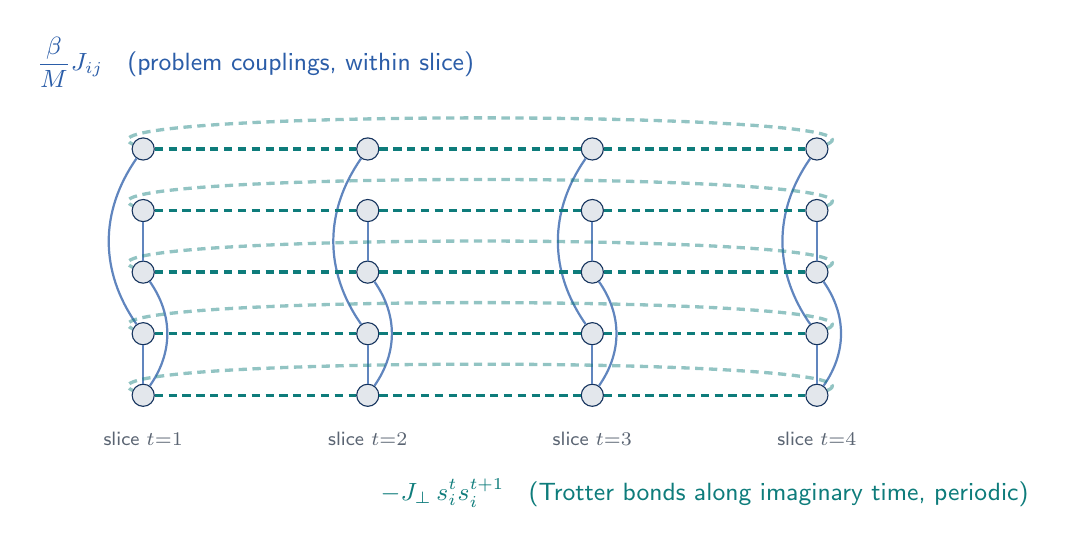
\begin{tikzpicture}[scale=0.92,
  spin/.style={circle,draw=qnavy,fill=qnavy!12,inner sep=1.6pt,minimum size=8pt},
  intra/.style={qblue!75,thick},
  inter/.style={qteal,very thick,densely dashed}]
% slices: 4 slices x 5 spins
\foreach \t in {0,1,2,3}{
  \begin{scope}[shift={(\t*3.1,0)}]
    \foreach \i in {0,...,4}{ \node[spin] (s\t\i) at (0,\i*0.85) {}; }
    % intra-slice couplings (a few representative)
    \draw[intra] (s\t0) to[bend right=35] (s\t2);
    \draw[intra] (s\t1) to[bend left=35] (s\t4);
    \draw[intra] (s\t2) -- (s\t3);
    \draw[intra] (s\t0) -- (s\t1);
    \node[below=2mm of s\t0,font=\scriptsize\sffamily\color{qgray}]
      {slice $t{=}\pgfmathparse{int(\t+1)}\pgfmathresult$};
  \end{scope}}
% inter-slice bonds
\foreach \t/\tn in {0/1,1/2,2/3}{
  \foreach \i in {0,...,4}{ \draw[inter] (s\t\i) -- (s\tn\i); }}
% periodic wrap
\foreach \i in {0,...,4}{
  \draw[inter,opacity=0.45] (s3\i) .. controls +(1.2,0.55) and +(-1.2,0.55) .. (s0\i);}
% labels
\node[font=\small\sffamily\color{qblue}] at (1.55,4.6)
  {$\dfrac{\beta}{M}J_{ij}$ \; (problem couplings, within slice)};
\node[font=\small\sffamily\color{qteal}] at (7.75,-1.35)
  {$-\Jp\, s^t_i s^{t+1}_i$ \; (Trotter bonds along imaginary time, periodic)};
\end{tikzpicture}
\caption{The Suzuki--Trotter mapping: $M$ replicas of the classical problem
(here $M{=}4$, $n{=}5$) coupled site-by-site along a periodic imaginary-time
ring. The row of same-site spins across all slices is that site's
\emph{worldline}.}
\label{fig:trotter}
\end{figure}

\subsection{Trotter error and choosing $M$}

The systematic error of the discretisation is $O\!\left((\beta\Gamma/M)^2\right)$
per slice. In practice:
\begin{itemize}
\item $M=16$--$32$ (the default is 32) suffices for optimisation use, where
we care about ground-state \emph{identification} rather than unbiased
thermodynamics.
\item Increase $M$ if the per-slice energies disagree strongly with each
other late in the anneal (a Trotter-error signature), or when running at
large $\beta\Gamma$.
\item Memory and time grow linearly in $M$; the OpenMP path parallelises
over replicas and slices, softening the wall-clock cost.
\item \code{continuous\_time\_slices > 0} overrides $M$ with a much larger
value to approximate the continuous-time limit within the discrete engine;
the genuinely continuous algorithm is Chapter~\ref{ch:ctpimc}.
\end{itemize}

\section{Monte Carlo moves on the Trotter system}
\label{sec:sqa-moves}

The \code{SQAAnnealer} mixes three move types, each preserving detailed
balance for the action Eq.~\eqref{eq:action}. Every acceptance test is
$\min(1,\mathrm{e}^{-\Delta S})$; what differs is the update and its
$\Delta S$.

\subsection{Single-spin (slice) moves}

Flip one spin $s^t_i$. The action change has a classical part within the
slice and a quantum part from the two adjacent time-bonds:
\begin{keyeq}[Single-spin action change]
\begin{equation}
\Delta S=\frac{\beta}{M}\,\Delta\Ecl
\;+\;2\,\Jp\,s^t_i\bigl(s^{t-1}_i+s^{t+1}_i\bigr),
\qquad \Delta\Ecl=-2\,s^t_i f^t_i ,
\label{eq:sqa-flip}
\end{equation}
\end{keyeq}
where $f^t_i$ is the cached local field of slice $t$
(Eq.~\eqref{eq:deltaE}). Both pieces are $O(1)$; the implementation keeps
one local-field cache per (replica, slice). \code{sweeps\_per\_beta} counts
these sweeps.

\subsection{Worldline moves}

Flip site $i$ in \emph{every} slice simultaneously
($s^t_i\to-s^t_i\ \forall t$). All imaginary-time bonds
$s^t_is^{t+1}_i$ are products of two flipped spins and are therefore
\emph{invariant}: the Trotter term cancels exactly, leaving
\begin{equation}
\Delta S_{\text{worldline}}=\frac{\beta}{M}\sum_{t=1}^{M}\Delta\Ecl^{(t)} .
\label{eq:worldline}
\end{equation}
Worldline moves are the quantum analogue of a classical single-spin flip and
are essential late in the anneal: when $\Jp$ is large the slices are locked
and single-slice flips are strongly suppressed
($\Delta S\approx4\Jp$), while a worldline flip pays no Trotter penalty at
all. \code{worldline\_sweeps} (default 5 in \code{solve()}) counts these.

\subsection{Swendsen--Wang cluster moves along imaginary time}
\label{sec:sw-moves}

Between the two extremes sits the cluster move: flip a \emph{contiguous
segment} of a worldline. Segments are grown stochastically with the
Fortuin--Kasteleyn rule specialised to the 1-D ferromagnetic time-chain of
coupling $\Jp$: starting from a random seed $(i,t)$, extend the cluster
across an aligned time-bond with the \emph{join probability}

\begin{keyeq}[Cluster join probability]
\begin{equation}
p_{\text{join}}=1-\mathrm{e}^{-2\Jp}.
\label{eq:joinprob}
\end{equation}
\end{keyeq}

Bonds inside the cluster then flip for free (the FK construction makes the
grown-bond factor cancel from the acceptance ratio); the remaining action
change --- the classical part in every touched slice plus the two
\emph{boundary} time-bonds where the cluster ends --- is Metropolis-tested:
\begin{equation}
\Delta S_{\text{cluster}}
=\frac{\beta}{M}\!\!\sum_{t\in\text{cluster}}\!\!\Delta\Ecl^{(t)}
\;+\;2\,\Jp\!\!\sum_{\text{boundary bonds}}\!\! s\,s' .
\end{equation}
Cluster moves interpolate smoothly between single-spin flips (clusters of
size 1 when $\Jp$ is small) and full worldline flips (system-spanning
clusters when $\Jp$ is large), and dramatically improve mixing in stiff,
strongly-coupled regimes. \code{cluster\_sweeps} (default 0) counts these;
setting it $>0$ is referred to as the \emph{+SW} variant of an engine.

\begin{notebox}[Which moves to enable]
A robust general-purpose mix is
\code{sweeps\_per\_beta=20--60}, \code{worldline\_sweeps=3--5},
\code{cluster\_sweeps=0}; add \code{cluster\_sweeps=1} for strongly
frustrated instances or whenever convergence visibly stalls at late steps.
All three counters multiply runtime linearly.
\end{notebox}

\section{The annealing loop and replicas}

Putting it together, \code{SQAAnnealer.run()} executes, for each schedule
step $(\beta_k,\Gamma_k)$:
\begin{enumerate}
\item recompute $\Jp(\beta_k,\Gamma_k,M)$ (Eq.~\eqref{eq:jperp}) and the
slice temperature factor $\beta_k/M$;
\item run the configured number of slice, worldline, and cluster sweeps with
the acceptance rules of Section~\ref{sec:sqa-moves};
\item measure the energy of \emph{every slice} of every replica; record the
best classical projection seen so far.
\end{enumerate}

The \code{replicas} parameter runs $R$ independent copies of the whole
Trotter system inside one call (OpenMP-parallel, one RNG stream per replica).
Besides restart statistics, replicas are what powers the adaptive schedule's
susceptibility estimator (Chapter~\ref{ch:optimal}), which pools samples
across them.

At the end, the returned \code{best\_state} is the best single \emph{slice}
ever observed --- the ``classical projection'' of the quantum state --- with
\code{best\_energy} its true classical energy $\Ecl$, and
\code{energy\_trace} the per-step mean energy.

\section{Usage}

\subsection{One-call interface}

\begin{pycode}
from qanneal import solve

result = solve(
    ising,
    method="sqa",
    reads=16,             # independent restarts
    trotter_slices=32,    # M
    replicas=4,           # parallel Trotter systems per read
    sweeps_per_beta=60,
    worldline_sweeps=4,
    cluster_sweeps=1,     # enable SQA+SW
    seed=42,
)
print(result.best_energy, result.best_sample)
\end{pycode}

\subsection{Explicit schedules}

If no schedule is given, \code{solve()} builds a tuned one
(Section~\ref{sec:sqa-tuned}). To control it explicitly:

\begin{pycode}
import numpy as np
from qanneal import SQASchedule, SQAAnnealer

schedule = SQASchedule.from_vectors(
    betas  = np.linspace(0.1, 5.0, 80).tolist(),
    gammas = np.geomspace(5.0, 0.01, 80).tolist(),   # geometric decay!
)
ann = SQAAnnealer(ising, schedule, trotter_slices=32, replicas=4)
ann.set_seed(7)
res = ann.run(sweeps_per_beta=60, worldline_sweeps=4, cluster_sweeps=1)
print(res.best_energy)
\end{pycode}

\begin{warnbox}[Use geometric $\Gamma$ decay]
$\Jp$ depends on $\Gamma$ logarithmically at small $\Gamma$
(Eq.~\eqref{eq:jperp}), so a \emph{linear} $\Gamma$ ramp spends most of its
steps in a narrow band of $\Jp$ and rushes the physically important region.
Geometric decay (\code{np.geomspace}) distributes steps roughly uniformly in
$\ln\Gamma$, i.e.\ far more evenly in $\Jp$.
\end{warnbox}

\subsection{Problem-adaptive tuned SQA schedules}
\label{sec:sqa-tuned}

\code{auto\_schedule\_sqa\_tuned(problem, mode=...)} extends the SA tuner of
Section~\ref{sec:tuned-schedules}: the same random-flip probe estimates the
energy scale $\Delta$, then
\begin{equation}
\Gamma_{\text{start}}=m_\Gamma\,\Delta,\qquad
\Gamma_{\text{end}}=\Gamma_{\text{start}}\cdot r_\Gamma\cdot
\code{gamma\_end\_scale},
\end{equation}
with $m_\Gamma\in\{2.0,\,3.0,\,4.5\}$ for
\code{fast}/\code{balanced}/\code{accurate} and geometric spacing in between.
$\beta$ ramps exactly as in the SA tuner. Setting
$\Gamma_{\text{start}}$ a few times the flip scale guarantees the run
actually begins in the quantum-disordered phase.

\begin{pycode}
from qanneal import auto_schedule_sqa_tuned
schedule = auto_schedule_sqa_tuned(ising, mode="balanced")
\end{pycode}

\section{Parameter summary}

\begin{center}
\small
\begin{tabular}{@{}llp{8.6cm}@{}}
\toprule
\textbf{Parameter} & \textbf{Default} & \textbf{Meaning}\\
\midrule
\code{trotter\_slices} & 32 & $M$; more slices $\Rightarrow$ less Trotter error, linearly more memory/time.\\
\code{replicas} & 1 & Independent Trotter systems per run (OpenMP-parallel). Use $\geq4$ with the optimal schedule.\\
\code{sweeps\_per\_beta} & 20 & Single-spin sweeps per schedule step.\\
\code{worldline\_sweeps} & 5 & Whole-worldline flips per step; essential at large $\Jp$.\\
\code{cluster\_sweeps} & 0 & Swendsen--Wang segment flips per step ($>0$ = SQA+SW).\\
\code{continuous\_time\_slices} & 0 & If $>0$, overrides $M$ to approximate continuous time.\\
\bottomrule
\end{tabular}
\end{center}

\chapter{Quantum Parallel Tempering (\code{sqapt})}
\label{ch:sqapt}

\code{sqapt} combines the two strongest ideas of the previous chapters:
the Suzuki--Trotter quantum simulation of Chapter~\ref{ch:sqa} and the
replica-exchange machinery of Section~\ref{sec:classical-pt}. It is the
\textbf{recommended default} for rugged, multi-modal problems: several
complete SQA systems run simultaneously at different points of a
$(\beta,\Gamma)$ ladder, and adjacent systems periodically swap
configurations so that solutions discovered under strong fluctuations flow
toward the strongly-frozen rungs where they are polished.

\section{The $(\beta,\Gamma)$ ladder}

Each of the $R$ replicas $r=1,\dots,R$ is a full Trotter system
($n\times M$ spins) equilibrating at its own pair $(\beta_r,\Gamma_r)$,
hence its own action $S_r$ (Eq.~\eqref{eq:action}) with its own
$\Jp^{(r)}=\Jp(\beta_r,\Gamma_r,M)$. The ladder is arranged so that mobility
decreases along it:

\begin{center}
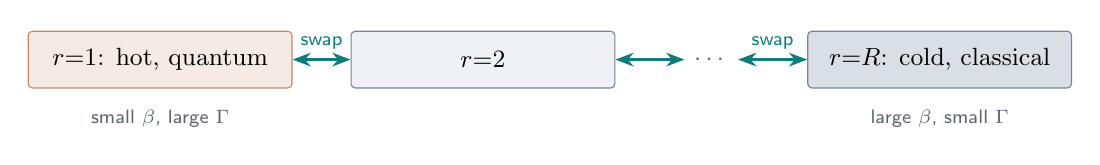
\begin{tikzpicture}[scale=1.0,
  rung/.style={rectangle,rounded corners=1.5pt,draw=qnavy!60,fill=qnavy!7,
               minimum width=3.35cm,minimum height=0.72cm,font=\small},
  sw/.style={{Stealth}-{Stealth},thick,qteal}]
\node[rung,fill=qamber!12,draw=qamber!70] (r1) at (0,0)
  {$r{=}1$: hot, quantum};
\node[rung] (r2) at (4.1,0) {$r{=}2$};
\node[font=\small\color{qgray}] (dots) at (7.0,0) {$\cdots$};
\node[rung,fill=qnavy!16] (rR) at (9.9,0) {$r{=}R$: cold, classical};
\draw[sw] (r1) -- node[above,font=\scriptsize\sffamily\color{qteal}]{swap} (r2);
\draw[sw] (r2) -- (dots);
\draw[sw] (dots) -- node[above,font=\scriptsize\sffamily\color{qteal}]{swap} (rR);
\node[below=1.5mm of r1,font=\scriptsize\sffamily\color{qgray}]
  {small $\beta$, large $\Gamma$};
\node[below=1.5mm of rR,font=\scriptsize\sffamily\color{qgray}]
  {large $\beta$, small $\Gamma$};
\end{tikzpicture}
\end{center}

\code{auto\_ladder\_sqa\_tuned(problem, replicas=R, mode=...)} builds the
ladder from the problem's probed energy scale:
\begin{itemize}
\item $\beta$ rungs are spaced \emph{geometrically} from
$\beta_{\min}$ (hot) to $\beta_{\max}$ (cold), so adjacent-rung energy
distributions overlap roughly uniformly along the ladder;
\item $\Gamma$ rungs are spaced \emph{inverse-geometrically} --- high
$\Gamma$ where $\beta$ is small, low $\Gamma$ where $\beta$ is large --- so
every rung sits at a physically coherent point (thermal and quantum mobility
rise and fall together).
\end{itemize}

\section{The quantum swap rule, derived}
\label{sec:quantum-swap}

The joint stationary measure is
$\Pi(\{x_r\})\propto\prod_r\mathrm{e}^{-S_r(x_r)}$, where $x_r$ denotes the
entire Trotter configuration of replica $r$ and
\begin{equation}
S_r(x)=\frac{\beta_r}{M}\sum_{t}\Ecl(s^t)\;-\;\Jp^{(r)}\sum_{t,i}s^t_i s^{t+1}_i
\;\equiv\;\frac{\beta_r}{M}\,C(x)\;-\;\Jp^{(r)}\,B(x),
\label{eq:action-cb}
\end{equation}
with $C(x)$ the summed classical energy over slices and $B(x)$ the total
imaginary-time \emph{bond sum}. (The quantity $B$ returns as the central
observable of Chapter~\ref{ch:optimal}.)

A swap proposes exchanging the full configurations of rungs $r$ and $r{+}1$.
Detailed balance for $\Pi$ gives the acceptance

\begin{keyeq}[SQAPT swap acceptance]
\begin{equation}
A_{\text{swap}}=\min\Bigl(1,\;
\exp\bigl[-\bigl(S_r(x_{r+1})+S_{r+1}(x_r)-S_r(x_r)-S_{r+1}(x_{r+1})\bigr)\bigr]\Bigr).
\label{eq:sqapt-swap}
\end{equation}
\end{keyeq}

This is precisely what the C++ core computes: it evaluates the four
cross-actions $S_r(x_r)$, $S_{r+1}(x_{r+1})$, $S_r(x_{r+1})$,
$S_{r+1}(x_r)$ from Eq.~\eqref{eq:action-cb} and applies
Eq.~\eqref{eq:sqapt-swap}. Expanding via Eq.~\eqref{eq:action-cb}, the
exponent splits into a thermal part and a quantum part:
\begin{equation}
\Delta_{\text{swap}}
=\frac{\beta_{r}-\beta_{r+1}}{M}\bigl(C(x_{r+1})-C(x_{r})\bigr)
\;-\;\bigl(\Jp^{(r)}-\Jp^{(r+1)}\bigr)\bigl(B(x_{r+1})-B(x_{r})\bigr).
\label{eq:swap-split}
\end{equation}
The first term is the classical PT criterion Eq.~\eqref{eq:pt-swap} applied
to slice-summed energies; the second exchanges configurations according to
their quantum ``kinetic'' content. When all replicas \emph{share} one
$\Jp$ --- as in the optimal-schedule mode of
Section~\ref{sec:sqapt-optimal} --- the second term vanishes identically and
the swap reduces to a purely classical criterion.

\section{The algorithm}

\code{SQAParallelTemperingAnnealer.run()} iterates \code{steps} epochs; in
each epoch every replica performs its local SQA updates
(\code{sweeps\_per\_step} single-spin sweeps, \code{worldline\_sweeps}
worldline sweeps, optionally \code{cluster\_sweeps} SW sweeps --- all with
the rules of Section~\ref{sec:sqa-moves} at that replica's own
$(\beta_r,\Gamma_r,\Jp^{(r)})$), and every \code{swap\_interval} epochs a
sweep of adjacent-pair swaps is attempted with
Eq.~\eqref{eq:sqapt-swap}. Replicas are OpenMP-parallel; the per-epoch swap
acceptance fraction is recorded in \code{swap\_acceptance\_trace}.

Unlike annealing, the ladder is \emph{static}: no schedule ramps during the
run. Optimisation progress comes from configurations drifting down the
ladder. The best classical projection (best single slice, any replica, any
epoch) is tracked exactly as in SQA.

\section{Usage}

\subsection{One call}

\begin{pycode}
from qanneal import solve

result = solve(
    ising,
    method="sqapt",
    replicas=8,          # ladder rungs
    reads=8,
    trotter_slices=24,
    sweeps_per_beta=50,  # local sweeps per epoch
    worldline_sweeps=4,
    cluster_sweeps=1,    # SQAPT+SW
    pt_steps=70,         # epochs
    swap_interval=1,
    seed=3,
)
\end{pycode}

If no schedule/ladder is supplied, \code{solve()} calls
\code{auto\_ladder\_sqa\_tuned} internally. Explicit ladders:

\begin{pycode}
from qanneal import auto_ladder_sqa_tuned, SQAParallelTemperingAnnealer

ladder = auto_ladder_sqa_tuned(ising, replicas=8, mode="balanced")
ann = SQAParallelTemperingAnnealer(
    ising, ladder.betas, ladder.gammas, trotter_slices=24)
res = ann.run(sweeps_per_step=50, worldline_sweeps=4,
              steps=80, swap_interval=1, cluster_sweeps=1)
print(res.best_energy)
print(res.swap_acceptance_trace[-5:])   # aim for ~0.2-0.5
\end{pycode}

You may also hand explicit ladders to \code{solve()} via
\code{pt\_betas=[...]}, \code{pt\_gammas=[...]} (they must pair up).

\subsection{Reading the diagnostics}

\begin{itemize}
\item \code{swap\_acceptance\_trace} --- mean accepted-swap fraction per
epoch. Healthy: $0.2$--$0.5$. Too low $\Rightarrow$ add rungs or narrow the
ladder; too high $\Rightarrow$ rungs redundant.
\item \code{final\_energies} --- final projected energy of each rung; should
be ordered roughly hot-to-cold. A cold rung stuck far above the best energy
signals insufficient epochs or a mobility bottleneck mid-ladder.
\item \code{average\_energy\_trace} --- ladder-mean energy per epoch;
plateaus indicate equilibration.
\end{itemize}

\section{Choosing \code{sqapt}}

\begin{itemize}
\item \textbf{Use it} for frustrated, glassy, multi-modal problems ---
anything where single-trajectory annealing shows large read-to-read
variance.
\item Ladder size \code{replicas}$\,=8$ is a solid default; scale up with
problem hardness, not with $n$.
\item \code{cluster\_sweeps=1} (SQAPT+SW) is the strongest general-purpose
configuration in the library.
\item Prefer \code{sqa} when the problem is easy enough that restarts
suffice --- SQAPT's ladder overhead ($R$ full Trotter systems) is then wasted.
\end{itemize}

The combination of \code{sqapt} with the adaptive $\Jp$ schedule --- a
shared, susceptibility-paced Trotter coupling ramp across the whole ladder ---
is covered in Section~\ref{sec:sqapt-optimal}.

\chapter{Continuous-Time PIMC (\code{ctpimc})}
\label{ch:ctpimc}

The fourth engine removes the Trotter discretisation altogether: it samples
the path integral directly in \emph{continuous} imaginary time, representing
each spin as a piecewise-constant \emph{worldline} on the circle
$[0,\beta)$. There is no Trotter error, and the cluster updates it employs
mix particularly well in the strongly quantum (large-$\Gamma$) regime. The
implementation builds on D-Wave's \code{localPIMC} code (Apache-2.0,
credited in \code{NOTICE}).

\section{From $M\to\infty$ to worldlines}

Recall the discrete action Eq.~\eqref{eq:action}. Take
$M\to\infty$ at fixed $\beta$: the slice index becomes a continuous
imaginary time $\tau\in[0,\beta)$ and each site's spin becomes a function
$s_i(\tau)\in\{-1,+1\}$, periodic in $\tau$, changing value at a finite set
of \emph{kinks} (domain walls in time). In this limit:

\begin{itemize}
\item The classical term becomes an integral,
$\frac{\beta}{M}\sum_t\Ecl(s^t)\;\longrightarrow\;\int_0^\beta
\Ecl\bigl(s(\tau)\bigr)\,d\tau$.
\item The Trotter bonds become a \emph{kink fugacity}: each kink on a
worldline carries a weight $\propto\Gamma\,d\tau$, i.e.\ in the absence of
couplings the kinks of site $i$ form a \emph{Poisson process} of rate
$\Gamma$ on the time circle.
\end{itemize}

\begin{keyeq}[Continuous-time path-integral weight]
\begin{equation}
Z=\sum_{\text{worldline configs}}
\;\Gamma^{\,K}\,
\exp\!\left[-\int_0^\beta \Ecl\bigl(s(\tau)\bigr)\,d\tau\right],
\end{equation}
where $K$ is the total number of kinks and the ``sum'' is over all
piecewise-constant periodic $\{s_i(\tau)\}$.
\end{keyeq}

Large $\Gamma$ favours many kinks (strong quantum fluctuation, rapidly
flapping worldlines); $\Gamma\to0$ suppresses kinks and worldlines freeze
into constants --- the classical configurations.

\section{Cluster updates on worldlines}

The engine updates worldlines with Swendsen--Wang-style cluster moves over
worldline \emph{segments} (the intervals between kinks): segments of
neighbouring sites are stochastically bound together according to the
couplings acting during their overlap in time, and bound clusters are
flipped as a unit. Kinks are created and removed in the process, so both the
spin values and the kink structure are resampled. This is the
continuous-time analogue of the discrete SW move of
Section~\ref{sec:sw-moves}, without any discretisation scale.

Two knobs shape the proposals:
\begin{itemize}
\item \code{qubits\_per\_update} --- how many sites participate in one
cluster proposal (1 = single-site updates);
\item \code{qubits\_per\_chain} --- chain length for the multi-site chain
updates used by the lattice mode.
\end{itemize}

\section{General mode}

For arbitrary \code{DenseIsing}/\code{SparseIsing} problems the annealer
follows a standard $(\beta,\Gamma)$ schedule. At each schedule step the
couplings are rescaled to the dimensionless combinations the sampler
consumes,
\begin{equation}
\beta J_{ij},\qquad \beta h_i,\qquad \beta\Gamma ,
\end{equation}
then \code{sweeps\_per\_beta} cluster sweeps are run and the classical
projection of the current worldlines is recorded. Reported energies are
converted back to the \emph{original} Ising units (not scaled by $\beta$).

\begin{pycode}
import numpy as np
from qanneal import DenseIsing, SQASchedule, CTPIMCAnnealer

h = np.array([0.2, -0.3, 0.1])
J = np.array([[0.0, -1.0, 0.2],
              [-1.0, 0.0, 0.5],
              [ 0.2, 0.5, 0.0]])
ising = DenseIsing(h, J)

schedule = SQASchedule.from_vectors(
    betas  = np.linspace(0.5, 4.0, 40).tolist(),
    gammas = np.linspace(2.0, 0.05, 40).tolist(),
)
annealer = CTPIMCAnnealer(ising, schedule,
                          qubits_per_update=1, qubits_per_chain=1)
res = annealer.run(sweeps_per_beta=50, reads=4)
print(res.best_energy)
\end{pycode}

Through the high-level interface:

\begin{pycode}
result = solve(ising, method="ctpimc", reads=8,
               ctpimc_qubits_per_update=1)
\end{pycode}

\begin{warnbox}[$\Gamma$ must stay positive]
The continuous-time weight is singular at $\Gamma=0$ (zero kink rate: the
sampler cannot move). End the schedule at a small positive value
(e.g.\ $10^{-3}$), never exactly zero. When building tuned schedules for
CT-PIMC, pass \code{gamma\_end\_scale=0.04} to
\code{auto\_schedule\_sqa\_tuned} so the final $\Gamma$ is near-zero for a
clean classical projection, yet finite.
\end{warnbox}

\section{Lattice mode}

A second constructor reproduces the cylindrical-lattice experiments the
underlying sampler was designed for (triangular and square-octagonal
geometries):

\begin{pycode}
from qanneal import CTPIMCAnnealer

annealer = CTPIMCAnnealer(
    Lperiodic=12,          # lattice period (multiple of 6)
    inv_temp_over_J=2.0,   # beta / J
    gamma_over_J=0.6,      # Gamma / J
    initial_condition=0,   # 0 random, 1 ferro, -1 antiferro
    qubits_per_update=1,
    qubits_per_chain=1,
)
res = annealer.run(sweeps_per_beta=32768)
\end{pycode}

Here temperatures and fields are expressed in units of the lattice coupling
$J$, and reported energies are likewise in units of $J$.

\section{CT-PIMC versus SQA}

\begin{center}
\small
\begin{tabular}{@{}lll@{}}
\toprule
 & \textbf{SQA (Chapter~\ref{ch:sqa})} & \textbf{CT-PIMC}\\
\midrule
Imaginary time & $M$ discrete slices & continuous\\
Systematic error & $O(\beta^2\Gamma^2/M)$ Trotter error & none\\
Elementary move & spin / worldline / SW segment & worldline-segment clusters\\
High-$\Gamma$ mixing & needs large $M$ & natural regime\\
Replica / PT structure & yes (\code{sqapt}) & no\\
Sweep-level observers & yes & no\\
\bottomrule
\end{tabular}
\end{center}

Use CT-PIMC when you want discretisation-free sampling closest in spirit to
physical-annealer statistics; use SQA/SQAPT when you need the replica
machinery, adaptive $\Jp$ schedules, or detailed observer traces. Neither
dominates the other on all problems.


\part{Adaptive Schedules}
\chapter{Adaptive Schedules from a Measured Susceptibility}
\label{ch:optimal}

Standard SQA follows a pre-designed $\Gamma(t)$ ramp fixed before the run
begins. Such a schedule cannot react to the system it is driving: it may
rush through the quantum critical region (exciting the system and spoiling
the solution) while wasting steps in regions where nothing interesting
happens. This chapter derives \qv's two alternatives: schedules that
\emph{measure} how critical the simulated system currently is --- through a
susceptibility $\chiB$ --- and pace the annealing trajectory accordingly.
They differ in their order parameter, their regularization, and their
execution model:

\begin{itemize}
\item \textbf{The optimal adaptive $\Jp$ schedule}
(Sections~\ref{sec:roland-cerf}--\ref{sec:optimal-diagnostics}) drives the
Trotter coupling $\Jp$ directly by the local adiabaticity ODE
$d\Jp/dt=\epst\,\chiB^{-\alpha}$, with $\chiB=\operatorname{Var}(B)$ the
susceptibility of the imaginary-time bond sum $B$. Available for \code{sqa}
and \code{sqapt}
(with or without SW cluster moves) via \code{schedule\_type="optimal"}.
\item \textbf{The worldline-magnetization susceptibility schedule}
(Section~\ref{sec:sqa-chi}) instead allocates the fixed step budget over
the annealing parameter $s$ by a floor-regularized weight
$w(s)=\max(\chiB(s),\text{floor})$, where $\chiB$ is now the susceptibility
of the worldline \emph{magnetization} $m$. It is a standalone solver
\emph{method}, \code{method="sqa\_chi"} --- not a \code{schedule\_type} of
\code{sqa} --- with its own parity-parallel update kernel.
\end{itemize}

Section~\ref{sec:sqa-chi-vs-optimal} compares the two directly.

\section{Local adiabaticity: the Roland--Cerf condition}
\label{sec:roland-cerf}

The adiabatic theorem (Section~\ref{sec:qa}) bounds the \emph{total} runtime
by the worst-case gap, Eq.~\eqref{eq:adiabatic}. Roland and
Cerf~\cite{rolandcerf} sharpened this into a \emph{local} condition: rather
than sweeping the control parameter uniformly, demand that the
\emph{instantaneous} transition probability stay uniformly small. For a
control parameter $\lambda(t)$ this reads
\begin{equation}
\Bigl|\frac{d\lambda}{dt}\Bigr|
\;\le\;\eps\,
\frac{\Delta_{\mathrm{gap}}^2(\lambda)}{\bigl|\bra{1}\partial_\lambda\hat H\ket{0}\bigr|}
\;\;\sim\;\;\eps\,\Delta_{\mathrm{gap}}^2(\lambda),
\label{eq:local-adiabatic}
\end{equation}
with $\eps\ll1$ a fixed error budget. The schedule then \emph{slows down
exactly where the gap is small} --- near the quantum critical point --- and
accelerates where the gap is large. For the archetypal Grover problem this
converts the naive $O(1/\Delta_{\min}^2)$ total time into the provably
optimal $O(1/\Delta_{\min})$; generically it redistributes a fixed time
budget in the provably best way.

\subsection{From the gap to a measurable quantity}

Eq.~\eqref{eq:local-adiabatic} is not directly usable: the gap of an
$n$-spin system is unknown. But near a second-order quantum phase
transition, \emph{finite-size scaling} links the gap to correlation
functions that Monte Carlo can measure. With correlation length $\xi$,
dynamical exponent $z$ and anomalous dimension $\eta$:
\begin{equation}
\Delta_{\mathrm{gap}}\sim\xi^{-z},
\qquad\qquad
\chi\;\sim\;\xi^{\,2-\eta},
\end{equation}
where $\chi$ is the susceptibility of the operator driving the transition.
Eliminating $\xi$:
\begin{equation}
\Delta_{\mathrm{gap}}^2 \;\sim\; \chi^{-2z/(2-\eta)} .
\end{equation}
In the Suzuki--Trotter representation the natural control parameter is the
Trotter coupling $\Jp$ (Eq.~\eqref{eq:jperp}) and the natural susceptibility
is that of the quantity $\Jp$ multiplies in the action
Eq.~\eqref{eq:action-cb}: the total imaginary-time \textbf{bond sum}
\begin{keyeq}[Bond sum and bond susceptibility]
\begin{equation}
B=\sum_{t=1}^{M}\sum_{i=1}^{n} s^t_i\,s^{t+1}_i,
\qquad\qquad
\chiB=\operatorname{Var}(B)=\langle B^2\rangle-\langle B\rangle^2 .
\label{eq:chiB}
\end{equation}
\end{keyeq}
$B$ plays the role of the conjugate ``order parameter density'' of the
transverse-field-driven transition; $\chiB$ is cheap to track (see
Section~\ref{sec:chib-est}) and peaks near the quantum transition.
Substituting into Eq.~\eqref{eq:local-adiabatic} and absorbing an extra
$+\tfrac12$ in the exponent that accounts for the statistical width of the
finite-sample variance estimator, the discrete update per adaptive step
becomes

\begin{keyeq}[Adaptive update law]
\begin{equation}
\Delta\Jp \;=\; \epst\cdot\chiB^{-\alpha},
\qquad\qquad
\alpha=\frac{z}{2-\eta}+\frac12 .
\label{eq:update-law}
\end{equation}
\end{keyeq}

For the 1-D quantum Ising universality class ($z=1$, $\eta=\tfrac14$):
$\alpha=\frac{1}{7/4}+\frac12=\frac{4}{7}+\frac12=\frac{15}{14}\approx1.071$
--- the library default (\code{optimal\_alpha}). For the 2-D class use
$\alpha=7/4$; for mean-field (Sherrington--Kirkpatrick-like) problems
$\alpha\approx1$ is a reasonable, if tentative, choice. In practice
$15/14$ is a robust default even when the true universality class is
unknown, because the calibration below makes the schedule's overall pace
independent of moderate errors in $\alpha$.

\begin{physbox}
For this model $\chiB$ is \emph{large near the quantum transition and
collapses toward zero deep in the ordered (classical) phase} --- it peaks
rather than diverging. Through Eq.~\eqref{eq:update-law} the schedule
therefore takes small steps ($\chiB$ large) in the critical window and large
steps ($\chiB$ small) once the system has ordered: a characteristic
\textbf{fast--slow--fast} trajectory in $\Jp$, dwelling exactly where
diabatic errors would otherwise be created.
\end{physbox}

\begin{figure}[ht]
\centering
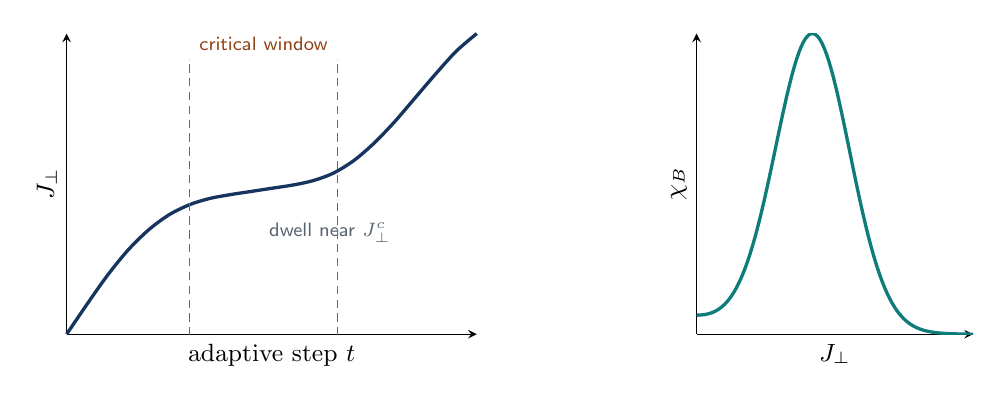
\begin{tikzpicture}
\begin{axis}[
  width=0.56\textwidth,height=5.4cm,
  xlabel={adaptive step $t$},ylabel={$\Jp$},
  axis lines=left,ticks=none,
  every axis label/.append style={font=\small},clip=false]
\addplot[qnavy,very thick,smooth] coordinates {
  (0,0.1) (0.05,2.5) (0.10,4.8) (0.15,6.8) (0.20,8.4) (0.25,9.6)
  (0.30,10.4) (0.35,10.9) (0.40,11.2) (0.45,11.45) (0.50,11.7)
  (0.55,11.95) (0.60,12.3) (0.65,12.9) (0.70,13.9) (0.75,15.3)
  (0.80,17.0) (0.85,18.9) (0.90,20.8) (0.95,22.6) (1.0,24.0)};
\node[font=\scriptsize\sffamily\color{qgray},anchor=west] at (axis cs:0.47,8.2)
  {dwell near $\Jp^{c}$};
\draw[qamber,densely dashed] (axis cs:0.30,0) -- (axis cs:0.30,22);
\draw[qamber,densely dashed] (axis cs:0.66,0) -- (axis cs:0.66,22);
\node[font=\scriptsize\sffamily\color{qamber!80!black}] at (axis cs:0.48,23.2)
  {critical window};
\end{axis}
\begin{scope}[shift={(8.0,0)}]
\begin{axis}[
  width=0.42\textwidth,height=5.4cm,
  xlabel={$\Jp$},ylabel={$\chiB$},
  axis lines=left,ticks=none,
  every axis label/.append style={font=\small},
  domain=0:1,samples=120]
\addplot[qteal,very thick] {exp(-((x-0.42)^2)/(2*0.018)) + 0.06*exp(-3*x)};
\node[font=\scriptsize\sffamily\color{qgray}] at (axis cs:0.42,1.12)
  {peak at $\Jp^{c}\!\approx\! J_{\mathrm{rms}}$};
\end{axis}
\end{scope}
\end{tikzpicture}
\caption{Schematic of a healthy adaptive run. Left: the realised
$\Jp(t)$ is fast--slow--fast, dwelling in the critical window. Right: the
bond susceptibility $\chiB(\Jp)$ that drives the pacing, peaking near the
quantum transition and collapsing in the ordered phase.}
\label{fig:fastslow}
\end{figure}

\section{Budget calibration: fixing the scale of \texorpdfstring{$\epst$}{eps-tilde}}
\label{sec:calibration}

Eq.~\eqref{eq:update-law} separates cleanly into \emph{shape} and
\emph{scale}: the factor $\chiB^{-\alpha}$ dictates \emph{where} the schedule
is slow or fast, while $\epst$ only sets the overall pace. Choosing
$\epst$ by hand is fragile: since $\chiB$'s magnitude grows with $n$, $M$
and the coupling distribution, a value that works for one instance can make
another instance's schedule either leap across its whole range in a few
steps or --- the more insidious failure --- \emph{freeze}, advancing $\Jp$ so
slowly that the run effectively anneals at constant coupling. Neither
failure announces itself: the run completes and returns an energy.

\qv{} therefore ties $\epst$ to the \emph{step budget}. Treat
Eq.~\eqref{eq:update-law} as an ODE in continuous step-time,
$\frac{dJ}{dt}=\epst\,\chiB(J)^{-\alpha}$, and separate variables:
$dt=\epst^{-1}\chiB(J)^{\alpha}\,dJ$. Requiring the traversal of
$[J_0,J_{\mathrm{end}}]$ to take \emph{exactly} $T=\code{num\_steps}$ steps,
\begin{equation}
T=\frac{1}{\epst}\int_{J_0}^{J_{\mathrm{end}}}\chiB(J)^{\alpha}\,dJ
\end{equation}

\begin{keyeq}[Budget-calibrated adiabaticity scale]
\begin{equation}
\epst \;=\; \frac{1}{T}\int_{J_0}^{J_{\mathrm{end}}}\chiB(J)^{\alpha}\,dJ .
\label{eq:calibrated-eps}
\end{equation}
\end{keyeq}

\begin{warnbox}[Sign of the exponent]
Note the \emph{positive} power $\chiB^{+\alpha}$ inside the integral and the
$1/T$ prefactor. The superficially plausible alternative
$\epst=\Delta\Jp/\sum_m\chiB(J_m)^{-\alpha}$ (negative power, no $1/T$) is
\emph{not} budget-correct when $\chiB$ varies along the range --- it under- or
over-shoots and can re-freeze the schedule. Eq.~\eqref{eq:calibrated-eps}
follows uniquely from the separation of variables above.
\end{warnbox}

\subsection{The pilot pre-pass}

$\chiB(J)$ is not known in advance, so when \code{eps\_tilde}\,$\le0$
(the default \code{optimal\_eps\_tilde=0.0} requests exactly this)
\code{run\_optimal} first runs a short \emph{pilot}: it measures $\chiB$ at
\code{calib\_probes} (default 12) values of $\Jp$ spanning
$[J_0,J_{\mathrm{end}}]$, using \code{calib\_sweeps} (default 10) sweeps per
probe with the \emph{same} sampler the real run will use, on scratch states
so the production run is unbiased. The integral in
Eq.~\eqref{eq:calibrated-eps} is then evaluated by the midpoint rule over
the probe grid.

\subsection{The inverse-CDF trajectory}

One more robustness step: rather than integrating
Eq.~\eqref{eq:update-law} \emph{online} with the noisy within-run $\chiB$
(whose fluctuations can compound --- a run that momentarily orders faster than
the pilot predicted sees a small $\chiB$, takes a huge step, and skips the
rest of the range), the entire trajectory is \emph{precomputed} from the
pilot profile. Define the cumulative ``adiabatic cost''
\begin{keyeq}[Inverse-CDF placement of steps]
\begin{equation}
G(J)=\int_{J_0}^{J}\chiB(J')^{\alpha}\,dJ' ,
\qquad\qquad
J^{(t)}=G^{-1}\!\Bigl(\frac{t}{T-1}\,G(J_{\mathrm{end}})\Bigr),
\quad t=0,\dots,T-1 .
\label{eq:inverse-cdf}
\end{equation}
\end{keyeq}
Each step is placed at an equal increment of adiabatic cost. By
construction --- independent of the shape or scale of $\chiB$ --- the schedule
(a)~consumes exactly $T$ steps, (b)~reaches $J_{\mathrm{end}}$, and
(c)~concentrates its steps where $\chiB$ is large. The online $\chiB$ is
still measured at every step and recorded in \code{chi\_B\_trace} as a
diagnostic (and, in the debug CSV, as \code{chi\_B\_online}).

A \emph{positive} \code{eps\_tilde} bypasses calibration entirely and drives
the legacy online update $\Jp\mathrel{+}=\epst\,\chiB^{-\alpha}$ with that
fixed scale --- retained for reproducibility and for controlled experiments,
not recommended for production.

\subsection{Fairness of the step budget}

The adaptive run \emph{always} executes all \code{num\_steps} steps; if
$\Jp$ saturates at $J_{\mathrm{end}}$ early it keeps sweeping at the
endpoint rather than stopping. Total sweep effort is therefore identical to
a standard-schedule run of the same length --- any quality difference is
attributable to the \emph{placement} of the steps, not to extra compute.

\section{Estimating \texorpdfstring{$\chiB$}{chi\_B} without overhead}
\label{sec:chib-est}

\subsection{Incremental bond tracking}

Recomputing $B$ (Eq.~\eqref{eq:chiB}) from scratch costs $O(nM)$; instead,
every move type updates it incrementally in $O(1)$ per flip:

\begin{center}
\small
\begin{tabular}{@{}lp{9.1cm}@{}}
\toprule
\textbf{Move} & \textbf{Bond-sum change $\Delta B$}\\
\midrule
Metropolis flip of $s^t_i$ &
$\Delta B=-2\,s^t_i\bigl(s^{t-1}_i+s^{t+1}_i\bigr)$ evaluated with the
\emph{old} spin value --- the two touched time-bonds reverse.\\
SW cluster flip &
$\Delta B=-2\sum_{\text{boundary bonds}} s\,s'$ --- only the bonds joining
the cluster to unflipped spins change; interior bonds are invariant.\\
Worldline flip &
$\Delta B=0$ --- every bond of the worldline is a product of two flipped
spins.\\
\bottomrule
\end{tabular}
\end{center}

After each full sweep the current $B$ is appended to the step's sample
buffer, so $\chiB$ estimation adds essentially zero cost to the run.

\subsection{Pooled variance across sweeps and replicas}

Each adaptive step yields $R\times S$ samples of $B$ ($R$ replicas,
$S$ sweeps within the step), pooled into one estimate
$\chiB=\widehat{\operatorname{Var}}(B)$. The pooling is statistically
well-behaved in both regimes:
\begin{itemize}
\item \emph{Near criticality}, the autocorrelation time
$\tau_{\mathrm{int}}\gg S$, so each replica's $S$ samples are nearly
identical and the pooled variance collapses to the \emph{cross-replica}
variance --- exactly the honest estimator for correlated chains.
\item \emph{Away from criticality}, $\tau_{\mathrm{int}}\ll S$ and the
pooled estimate enjoys $\sim RS$ effectively independent samples.
\end{itemize}
This is the reason \code{replicas}\,$\geq4$ is recommended whenever
\code{schedule\_type="optimal"} is used.

\subsection{Single-replica guard and the \texorpdfstring{$\chiB$}{chi-B} floor}

Two safeguards prevent pathological steps:
\begin{description}
\item[$R=1$ guard.] With a single replica near criticality all within-step
samples coincide, the naive variance $\to0$, and
Eq.~\eqref{eq:update-law} would take its \emph{maximum} step precisely where
it must be smallest. The implementation therefore uses
$\chiB=\max\bigl(\widehat{\operatorname{Var}}(B),\;
nM\bigl[1-(B/nM)^2\bigr]\bigr)$, the second term being the
single-bond variance extrapolated over the lattice --- a strictly positive
lower bound near criticality.
\item[Floor.] Deep in the ordered phase $\chiB\to0$ and
$\chiB^{-\alpha}$ blows up; a floor
$\chiB\ge10^{-4}\max_J\chiB^{\text{(pilot)}}$ caps the step size. The debug
CSV records where the floor activates (\code{floor\_hit}); in a healthy run
this is only the deeply ordered tail, never the critical window.
\end{description}

\section{Endpoints, temperature, and the two-phase SQA protocol}
\label{sec:optimal-params}

\subsection{Choosing $J_0$ and $J_{\mathrm{end}}$}

All endpoints derive from the problem's own coupling scale. Let
\begin{equation}
J_{\mathrm{rms}}=\sqrt{\operatorname{mean}\bigl(J_{ij}^2\bigr)}
\quad\text{over the non-zero couplings}
\end{equation}
(computable via \code{j\_rms\_from\_problem(problem)}). The quantum critical
coupling scales as $\Jp^{c}\sim J_{\mathrm{rms}}$, so:
\begin{itemize}
\item \code{j\_perp\_start} --- from the tuned standard schedule's
$(\beta,\Gamma_{\text{start}})$ through Eq.~\eqref{eq:jperp}; small
(quantum end).
\item \code{j\_perp\_end} --- default $\max(J_0,\;5\,J_{\mathrm{rms}})$,
comfortably past the transition (classical end).
\item $\beta$ --- for SQA, $\beta=\max(4/J_{\mathrm{rms}},\,1)$, i.e.\ cold
enough that $\beta J_{\mathrm{rms}}\geq4$: thermal fluctuations must not
wash out the order the $\Jp$ ramp is trying to establish.
\end{itemize}
The helper returns all three at once:
\begin{pycode}
from qanneal import optimal_j_perp_params, j_rms_from_problem
beta, jp_start, jp_end = optimal_j_perp_params(problem, trotter_slices=32)
jr = j_rms_from_problem(problem)
\end{pycode}

\begin{warnbox}[When can the adaptive schedule help at all?]
The schedule needs a quantum range to act on: it helps when
$J_{\mathrm{rms}}\gtrsim\code{j\_perp\_start}$ (in the auto-tuned setting,
roughly $J_{\mathrm{rms}}\gtrsim3$), so that the run genuinely starts on the
disordered side of the transition. If $J_{\mathrm{rms}}$ is far below
$J_0$ the system is already effectively classical at step one,
$\chiB\approx0$ everywhere, and no schedule --- adaptive or not --- has
anything to optimise. Check a new problem class with
\code{scripts/sanity\_schedule.py}, which classifies instances as
\code{PASS} or \code{DEGENERATE} before you spend compute.
\end{warnbox}

\begin{warnbox}[Always pass an explicit \code{j\_perp\_end} in scripted runs]
The C++ \code{run\_optimal} accepts a sentinel \code{j\_perp\_end<=0}
that resolves to the coldest replica's Trotter coupling. If that resolves
\emph{below} \code{j\_perp\_start} the schedule has no range; the code then
installs a large fallback ceiling and prints a \code{cerr} warning. Relying
on the sentinel makes runs silently sensitive to ladder details --- pass an
explicit \code{j\_perp\_end} (e.g.\ $5J_{\mathrm{rms}}$) in anything
scripted.
\end{warnbox}

\subsection{Two-phase protocol for SQA}

Plain SQA under the adaptive schedule holds a \emph{single} fixed $\beta$
--- it has no thermal annealing at all, which measurably hurts it. The SQA
\code{run\_optimal} therefore runs two phases, split by
\code{beta\_ramp\_fraction} (default $0.3$):
\begin{enumerate}
\item \textbf{Thermal ramp} --- for the first
$\lceil0.3\cdot\code{num\_steps}\rceil$ steps, $\beta$ ramps from
\code{beta\_ramp\_start} (default $0.1$) up to the cold target
$\beta=\max(4/J_{\mathrm{rms}},1)$ at \emph{fixed} $\Jp=J_0$: a conventional
thermal anneal that settles the slices into the disordered quantum state at
the right temperature.
\item \textbf{Adaptive ramp} --- $\beta$ then stays fixed while $\Jp$
follows the calibrated inverse-CDF trajectory
Eq.~\eqref{eq:inverse-cdf} over the remaining steps.
\end{enumerate}
SQAPT does \emph{not} use phase 1: its $(\beta,\Gamma)$ ladder plus replica
swaps already supply thermal mobility.

\subsection{SQAPT under a shared $\Jp$}
\label{sec:sqapt-optimal}

In the SQAPT variant, \emph{all} rungs share the single evolving $\Jp$;
each keeps its own $(\beta_r,\Gamma_r)$ from the ladder. Two consequences,
both derived earlier:
\begin{itemize}
\item In the swap exponent Eq.~\eqref{eq:swap-split} the quantum term
carries the factor $\Jp^{(r)}-\Jp^{(r+1)}=0$: \textbf{swaps reduce to the
purely classical criterion} on slice-summed energies.
\item $\chiB$ is estimated by pooling $B$-samples across all rungs, exactly
as in Section~\ref{sec:chib-est}.
\end{itemize}

\section{Usage}

\subsection{High-level}

\begin{pycode}
from qanneal import solve

result = solve(
    problem,
    method="sqa",              # or "sqapt"
    schedule_type="optimal",
    reads=15,
    replicas=4,                # >=4 for a reliable chi_B estimate
    optimal_eps_tilde=0.0,     # 0.0 = per-instance budget calibration
    optimal_num_steps=150,
    # Optional overrides (auto-computed from the problem scale if omitted):
    # optimal_j_perp_end=25.0,         # default max(j_perp_start, 5*j_rms)
    # optimal_beta_ramp_fraction=0.3,  # SQA two-phase split
    # optimal_alpha=15/14,
    # optimal_debug_csv="schedule.csv" # per-step J_perp / chi_B diagnostics
)
print(result.best_energy, result.best_sample)
\end{pycode}

For SQAPT with SW cluster moves:

\begin{pycode}
result = solve(
    problem,
    method="sqapt",
    schedule_type="optimal",
    replicas=8, reads=15,
    trotter_slices=32,
    worldline_sweeps=3,
    cluster_sweeps=1,          # >0 = SQAPT+SW
    swap_interval=1,
    optimal_eps_tilde=0.0,
    optimal_num_steps=150,
)
\end{pycode}

\subsection{Low-level, with full diagnostics}

\begin{pycode}
from qanneal import SQAAnnealer, SQASchedule

dummy = SQASchedule.from_vectors([1.0], [1.0])  # construction only
ann = SQAAnnealer(ising, dummy, trotter_slices=32, replicas=4)

result = ann.run_optimal(
    beta=1.0,                    # phase-2 (cold) inverse temperature
    j_perp_start=0.1, j_perp_end=25.0,
    eps_tilde=0.0,               # <=0 -> budget calibration
    alpha=15/14, num_steps=150, sweeps_per_step=20,
    worldline_sweeps=3, cluster_sweeps=0,
    calib_probes=12, calib_sweeps=10,   # pilot grid
    beta_ramp_fraction=0.3,             # two-phase thermal ramp
)
result.j_perp_trace          # realised J_perp(t)
result.chi_B_trace           # online chi_B(t)
result.calibrated_eps_tilde  # the eps from Eq. (calibration)
result.final_j_perp          # J_perp actually reached
result.best_state, result.best_energy
\end{pycode}

The SQAPT twin is \code{SQAParallelTemperingAnnealer.run\_optimal}
(full signature in Chapter~\ref{ch:api}), with identical calibration
semantics and no two-phase ramp.

\section{Diagnosing a run}
\label{sec:optimal-diagnostics}

Plot the three traces after any adaptive run:

\begin{pycode}
import numpy as np, matplotlib.pyplot as plt

t  = np.arange(len(result.j_perp_trace))
dj = np.diff(result.j_perp_trace)

fig, axs = plt.subplots(3, 1, figsize=(8, 9), sharex=True)
axs[0].plot(t, result.j_perp_trace);  axs[0].set_ylabel("J_perp")
axs[1].plot(t[:-1], dj);              axs[1].set_ylabel("step size dJ_perp")
axs[2].plot(t, result.energy_trace);  axs[2].set_ylabel("energy")
axs[2].set_xlabel("adaptive step")
plt.suptitle("Optimal schedule diagnostics"); plt.tight_layout(); plt.show()
\end{pycode}

\textbf{A healthy run} shows (Fig.~\ref{fig:fastslow}): fast early movement,
a pronounced dwell (small $\Delta\Jp$) in the critical window near
$\Jp\approx J_{\mathrm{rms}}$, fast movement again past the transition, the
endpoint reached within budget, and the steepest energy descent during the
dwell.

\textbf{Warning signs:}
\begin{itemize}
\item \emph{Flat or linear $\Jp(t)$ with no dwell} --- the schedule is
frozen or degenerate. Check that $J_{\mathrm{end}}>J_0$ (look for the
\code{cerr} fallback warning) and that the problem is in the favourable
regime ($J_{\mathrm{rms}}\gtrsim J_0$).
\item \emph{Constant $\Delta\Jp$} --- $\chiB$ estimate too noisy to shape
the trajectory; raise \code{replicas} and/or \code{sweeps\_per\_step}.
\item \emph{\code{final\_j\_perp} far below \code{resolved\_j\_perp\_end}}
on a non-degenerate instance --- calibration failed; inspect the debug CSV
(columns \code{phase}, \code{step\_index}, \code{j\_perp}, \code{chi\_B},
\code{delta\_j}, \code{eps\_tilde}, \code{alpha}, \code{floor\_hit},
\code{chi\_B\_online}; \code{phase=calib} rows are pilot probes).
The helper \code{scripts/}\allowbreak\code{plot\_schedule\_trajectory.py}
renders it.
\end{itemize}

\begin{notebox}[Pre-flight habit]
Before any long or large-$n$ run, spend a minute on a small instance of the
same problem class: run with \code{optimal\_debug\_csv} set, plot the
trajectory, and confirm the fast--slow--fast shape.
\code{python scripts/sanity\_schedule.py --n 40 --steps 150 --plot}
automates exactly this check and prints \code{PASS} / \code{DEGENERATE} /
\code{FAIL} per instance.
\end{notebox}

\section{Attribution: schedule effect vs.\ cluster moves}
\label{sec:attribution}

The adaptive \emph{schedule} and SW \emph{cluster sweeps} are independent
mechanisms that both help on hard instances. When evaluating the schedule on
your own problems, keep them separate or you will misattribute gains:

\begin{center}
\small
\begin{tabular}{@{}lll@{}}
\toprule
\textbf{Comparison} & \textbf{\code{cluster\_sweeps}} & \textbf{Isolates}\\
\midrule
\code{sqapt}-std vs \code{sqapt}-opt & $0$ & the schedule effect alone\\
\code{sqapt}+SW-std vs \code{sqapt}+SW-opt & $>0$ & schedule $\times$ cluster interaction\\
\bottomrule
\end{tabular}
\end{center}

Only credit ``the optimal schedule'' if the first comparison reproducibly
favours it; if only the +SW pair improves, the gain belongs to the
interaction and should be framed as such.

\section{The worldline-magnetization susceptibility schedule
(\texorpdfstring{\code{sqa\_chi}}{sqa\_chi})}
\label{sec:sqa-chi}

The schedule above measures $\chiB$ from the imaginary-time bond sum $B$
and drives $\Jp$ online through \code{SQAAnnealer}. \qv{} 1.0.0 adds a
second, \emph{standalone} method built around a different order parameter
and a different execution model: \code{sqa\_chi} is not a
\code{schedule\_type} flag on \code{sqa} but its own solver class,
\code{SQAChiAnnealer}, generalized from a worldline-QMC validation script
into \qv's \code{Backend} abstraction (dense \emph{or} sparse Ising).

\subsection{Order parameter: the worldline magnetization}
\label{sec:sqa-chi-order-param}

Instead of the bond sum $B$ (Eq.~\eqref{eq:chiB}), \code{sqa\_chi} measures
the mean spin over the \emph{entire} worldline lattice of a replica ($n$
spins $\times\,M$ Trotter slices):
\begin{keyeq}[Worldline magnetization and its susceptibility]
\begin{equation}
m=\frac{1}{nM}\sum_{i=1}^{n}\sum_{k=1}^{M}\sigma_i^k,
\qquad\qquad
\chiB = nM\bigl(\langle m^2\rangle-\langle|m|\rangle^2\bigr),
\label{eq:chib-magnetization}
\end{equation}
\end{keyeq}
the ordinary classical-Ising susceptibility of the $(d{+}1)$-dimensional
Suzuki--Trotter lattice. Like $\operatorname{Var}(B)$, it peaks at the
quantum critical point --- both are measuring the growth of critical
fluctuations in the \emph{same} classical system, just through different
observables of it. $\langle\cdot\rangle$ pools every post-burn sweep sample
across all replicas, mirroring Section~\ref{sec:chib-est}'s pooling
(replicas $\ge4$ recommended for the same statistical reasons).

\subsection{The annealing parameter \texorpdfstring{$s$}{s}}

\code{sqa\_chi} works in the annealing parameter $s\in[0,1]$ of the
symmetric path $A(s)=A_0(1-s)$, $B(s)=s$ (driver and problem Hamiltonian
weights), rather than in $\Gamma$ directly:
\begin{keyeq}[Annealing parameter $\leftrightarrow$ transverse field]
\begin{equation}
s=\frac{A_0}{A_0+\Gamma},
\qquad\qquad
\Gamma=\frac{A_0(1-s)}{s},
\label{eq:sqa-chi-s}
\end{equation}
\end{keyeq}
so $s=0$ is the fully quantum end ($\Gamma\to\infty$) and $s=1$ the fully
classical end ($\Gamma=0$); the driver scale $A_0$ is \code{chi\_driver\_A0}
if positive, otherwise \code{gamma\_start}. This is a property of the
annealing \emph{path}, not of the $\chiB$ estimator --- the same relation
underlies every $s$-parametrized construction in \qv.

\subsection{Stage 1: the pilot \texorpdfstring{$\chiB(s)$}{chi\_B(s)} scan}

At \code{scan\_points} (default 16) uniform values of $s$ between
$s(\gamma_{\mathrm{start}})$ and $s(\gamma_{\mathrm{end}})$, the pilot runs
\code{scan\_burn}$+$\code{scan\_sweeps} (default $10+30$) parity-parallel
checkerboard sweeps (Section~\ref{sec:sqa-chi-kernel}) at the corresponding
fixed $\Jp$.

\begin{warnbox}[Fresh worldline per grid point --- deliberately not carried]
Unlike \code{run\_optimal}'s calibration pilot and the retired surrogate
schedule (both of which carry the worldline state between grid points so
the scan itself gently anneals), \code{sqa\_chi} starts every grid point
from a \emph{fresh, independently randomized} worldline. Each $\chiB(s)$
estimate is therefore a statistically independent measurement --- more
robust against carried-over bias between probes, at the cost of
re-equilibrating (\code{scan\_burn} sweeps) at every point.
\end{warnbox}

The scan profile (\code{scan\_s}, \code{scan\_gamma}, \code{scan\_chi\_B})
and the quantum critical point estimate --- the $\chiB$ peak, recorded as
(\code{s\_star}, \code{gamma\_star}, \code{j\_perp\_star}) --- are returned
as diagnostics.

\subsection{Stage 2: floor-regularized time allocation}

The pilot profile is turned into a floor-regularized weight and its
cumulative integral:
\begin{keyeq}[Floored weight and its cumulative integral]
\begin{gather}
w(s)=\max\bigl(\chiB(s),\,\text{floor}\bigr),
\qquad
\text{floor}=\max\Bigl(\code{chi\_floor\_fraction}\cdot\max_s\chiB(s),\,
10^{-12}\Bigr),
\label{eq:sqa-chi-weight}\\[4pt]
\tau(s)=\frac{\displaystyle\int_{s_{\mathrm{lo}}}^{s}w(s')\,ds'}
             {\displaystyle\int_{s_{\mathrm{lo}}}^{s_{\mathrm{hi}}}w(s')\,ds'} .
\end{gather}
\end{keyeq}
$\chiB(s)$ linearly interpolated between scan points (clamped to the
boundary value outside $[s_{\mathrm{lo}},s_{\mathrm{hi}}]$). Each of the
remaining (post-ramp) adaptive steps $k=0,\dots,n_2-1$ is placed at
$s_k=\tau^{-1}\!\bigl(k/(n_2-1)\bigr)$, evaluated on a fixed 4096-point grid
by trapezoidal integration and linear inversion, then mapped to
$\gamma_k=A_0(1-s_k)/s_k$ (clamped into
$[\gamma_{\mathrm{end}},\gamma_{\mathrm{start}}]$).

\begin{notebox}[A floor, not an additive regularizer]
The optimal schedule's calibration floor and the retired surrogate
schedule both use an \emph{additive} term ($\chiB+\chi_0$) to keep the
weight strictly positive. \code{sqa\_chi} instead \emph{clamps}
$\chiB$ from below --- a multiplicative floor, matching the reference
validation script's regularization idea (\code{np.maximum(chi\_B, eps)})
but generalized: the script's fixed absolute $\epsilon=10^{-8}$ is not
scale-invariant across problem sizes ($\chiB\sim O(nM)$), so \qv{} scales
the floor to a fraction of the scan's own peak instead.
\end{notebox}

\begin{notebox}[Degenerate profile]
If the pilot scan is flat or non-finite (no measurable $\chiB$ signal),
\code{floor} falls back to $1.0$ and a \code{cerr} warning is printed;
$w(s)$ is then constant and the schedule degrades gracefully to a
linear-in-$s$ ramp rather than failing.
\end{notebox}

\subsection{The parity-parallel checkerboard kernel}
\label{sec:sqa-chi-kernel}

Every sweep in \code{sqa\_chi} --- pilot \emph{and} production --- uses a
kernel that differs from every other engine in \qv{}: it parallelizes
\emph{within} a single replica's worldline, not just across replicas.

\begin{description}[style=nextline]
\item[The observation.] Trotter slices of the same parity (even/odd index)
are never directly coupled: the Trotter term only links slice $k$ to
$k\pm1$, which always belong to the \emph{other} parity. So while one
parity's slices are held fixed, every $(\text{replica},\text{slice})$ cell
of the other parity can be updated completely independently.
\item[The update.] Each cell runs a full, ordinary sequential single-spin
Metropolis sweep over its own $n$ spins, using the \code{Backend}'s cached
local fields (Section~\ref{sec:chib-est}'s $O(1)$/$O(\text{degree})$
incremental updates) --- exactly the update rule \code{SQAAnnealer} uses,
just scoped to one slice at a time.
\item[The parallelism.] All cells of one parity are dispatched to a single
OpenMP \code{\#pragma omp parallel for}, then the other parity, then the
lattice's pooled magnetization is read off. Two parity passes make one
full sweep.
\end{description}

\begin{warnbox}[Why not update a whole slice's spins simultaneously?]
A natural-looking shortcut --- flip every spin of a slice at once, using
the \emph{previous} sweep's neighbour values for the in-plane coupling ---
is what the reference validation script does. It is only exact detailed
balance when the spatial coupling graph is \emph{bipartite}; for a general
(dense or frustrated) Ising problem it silently biases the sampler. The
per-slice \emph{sequential} update above is exact for any coupling graph,
while still parallelizing across slices --- the price is that spins
\emph{within} one slice are still updated one at a time, not vectorised.
\end{warnbox}

Because the parallel axis is $(\text{replica}\times\text{slice})$ rather
than replica alone, \code{sqa\_chi} scales across cores even at
\code{replicas=1} — unlike every other SQA-family engine in \qv{}, whose
OpenMP parallelism is over replicas only and is therefore inert for a
single-replica run.

\subsection{Two-phase protocol and the main anneal}

As in Section~\ref{sec:optimal-params}, the first
$\lceil\code{beta\_ramp\_fraction}\cdot\code{num\_steps}\rceil$ steps ramp
$\beta$ from \code{beta\_ramp\_start} to the target $\beta$ at fixed
$\gamma=\gamma_{\mathrm{start}}$ (\code{beta\_ramp\_fraction}$\le0$ disables
this phase); the remaining steps hold $\beta$ fixed and follow the
$\gamma_k$ schedule from Stage 2. The resolved
(\code{beta\_schedule}, \code{gamma\_schedule}) is run on a \emph{fresh}
worldline (independent of the pilot scan's state, so the production run is
unbiased) through the same parity-parallel checkerboard kernel.

\subsection{Usage}

\begin{pycode}
from qanneal import solve

result = solve(
    problem,
    method="sqa_chi",                  # standalone method, not schedule_type="..."
    reads=15,
    replicas=4,                        # >=4 for a reliable chi_B estimate
    optimal_num_steps=150,             # shared step budget with schedule_type="optimal"
    chi_floor_fraction=1e-6,
    # Optional overrides (auto from the resolved standard schedule if omitted):
    # chi_gamma_start=5.0,             # default: max gamma of the tuned schedule
    # chi_gamma_end=0.01,              # default: min gamma of the tuned schedule
    # chi_scan_points=16, chi_scan_sweeps=30, chi_scan_burn=10,
    # chi_driver_A0=0.0,               # <=0 resolves to chi_gamma_start
    # optimal_beta_ramp_fraction=0.3,  # shared two-phase split
    # optimal_debug_csv="sqa_chi_schedule.csv",
)
print(result.best_energy, result.best_sample)
\end{pycode}

Low-level, with full diagnostics:

\begin{pycode}
from qanneal import SQAChiAnnealer

ann = SQAChiAnnealer(ising, trotter_slices=32, replicas=4)   # no schedule argument

result = ann.run_chi(
    beta=1.0, gamma_start=5.0, gamma_end=0.01,
    num_steps=150, sweeps_per_step=20,
    scan_points=16, scan_sweeps=30, scan_burn=10,
    chi_floor_fraction=1e-6, driver_A0=0.0,
    beta_ramp_fraction=0.3, beta_ramp_start=0.1,
)
result.scan_s, result.scan_gamma, result.scan_chi_B     # pilot chi_B(s) profile
result.s_star, result.gamma_star, result.j_perp_star    # QCP estimate
result.beta_schedule, result.gamma_schedule, result.s_schedule  # resolved trajectory
result.best_state, result.best_energy
\end{pycode}

\subsection{Diagnosing a run}

The same three-panel plot as Section~\ref{sec:optimal-diagnostics} applies
to \code{gamma\_schedule} / \code{s\_schedule} / \code{energy\_trace}; also
plot \code{scan\_chi\_B} against \code{scan\_s} to confirm the pilot found a
clear peak (a flat scan is the \code{sqa\_chi} analogue of a frozen
adaptive schedule --- see the degenerate-profile fallback above).

When \code{debug\_csv\_path} is set, columns are \code{phase}
(\code{scan}, \code{beta\_ramp}, or \code{run}), \code{index}, \code{s},
\code{gamma}, \code{j\_perp}, \code{chi\_B}, and \code{beta}; only
\code{scan} rows carry a measured \code{chi\_B} --- \code{beta\_ramp}/
\code{run} rows report the resolved schedule that \code{chi\_B} produced,
not an online remeasurement.

\subsection{\code{sqa\_chi} vs.\ the optimal \texorpdfstring{$\Jp$}{J-perp} schedule}
\label{sec:sqa-chi-vs-optimal}

\begin{center}
\small
\begin{tabular}{@{}p{2.6cm}p{6.0cm}p{6.0cm}@{}}
\toprule
& \textbf{Optimal $\Jp$ schedule} & \textbf{\code{sqa\_chi}}\\
\midrule
Exposed as & \code{schedule\_type="optimal"} on \code{sqa}/\code{sqapt} & standalone \code{method="sqa\_chi"}\\
Order parameter & bond sum $B=\sum_{k,i}\sigma_i^k\sigma_i^{k+1}$ & worldline magnetization $m=\text{mean}(\sigma)$\\
$\chiB$ formula & $\operatorname{Var}(B)$ & $nM(\langle m^2\rangle-\langle|m|\rangle^2)$\\
Control variable & $\Jp$ directly & $s$ (hence $\Gamma$)\\
Regularizer & multiplicative floor on $\chiB^{-\alpha}$ & multiplicative floor on $\chiB$ itself\\
Universality exponent & $\alpha$ required (default $15/14$) & none\\
Pilot-scan state & carried between grid points & fresh worldline per grid point\\
Update kernel & sequential per-slice, parallel over replicas & parity-parallel checkerboard over slices \emph{and} replicas\\
Parallel at \code{replicas=1}? & no & yes\\
Backends & dense or sparse & dense or sparse\\
Methods & \code{sqa}, \code{sqapt} (+SW) & \code{sqa\_chi} only\\
\bottomrule
\end{tabular}
\end{center}

Both precompute their trajectory from a pilot $\chiB$ profile rather than
integrating online, so neither is vulnerable to the compounding-noise
failure mode of Section~\ref{sec:calibration}. Treat the choice between
them as an empirical one: neither dominates the other on every instance,
and Section~\ref{sec:attribution} applies here as well --- isolate the
schedule effect from cluster-move effects (where applicable) before
crediting either one.


\part{Using the Library}
\chapter{Installation and Building}
\label{ch:install}

\section{Requirements}

\begin{center}
\small
\begin{tabular}{@{}lll@{}}
\toprule
\textbf{Component} & \textbf{Requirement} & \textbf{Role}\\
\midrule
Python & $\geq 3.11$ & front end\\
NumPy & any recent & array interchange\\
C++ compiler & C++17 (GCC $\geq9$, Clang $\geq10$, MSVC 2019+) & core engines\\
CMake & $\geq 3.18$ & build system (via scikit-build)\\
OpenMP & optional & parallel replicas/slices\\
MPI + \code{mpi4py} & optional & multi-node runs\\
\code{matplotlib}, \code{tqdm} & optional & plots, progress bars\\
\code{dimod}, \code{networkx} & optional & BQM / graph problem inputs\\
\bottomrule
\end{tabular}
\end{center}

\section{Installing the Python package}

From the repository root:

\begin{bashcode}
# Standard install (recommended)
python -m pip install . --no-build-isolation

# Editable install for development
python -m pip install -e . --no-build-isolation

# Convenience scripts
./setup.sh        # macOS / Linux
setup.bat         # Windows cmd
./setup.ps1       # Windows PowerShell
\end{bashcode}

The build compiles the C++17 core and the pybind11 extension
(\code{qanneal.\_qanneal}) in place. Verify:

\begin{bashcode}
python -c "import qanneal; print(qanneal.__version__)"   # 1.0.0
\end{bashcode}

\section{Building the C++ library directly}

For C++-only use, tests, or the MPI example:

\begin{bashcode}
cmake -S . -B build \
  -DQANNEAL_ENABLE_OPENMP=ON \
  -DQANNEAL_ENABLE_MPI=OFF \
  -DQANNEAL_BUILD_TESTS=ON \
  -DCMAKE_BUILD_TYPE=Release
cmake --build build -j
ctest --test-dir build
\end{bashcode}

\begin{center}
\small
\begin{tabular}{@{}llp{7.4cm}@{}}
\toprule
\textbf{CMake flag} & \textbf{Default} & \textbf{Effect}\\
\midrule
\code{QANNEAL\_ENABLE\_OPENMP} & \code{ON} & Parallel loops in Replica/SQA/SQAPT annealers.\\
\code{QANNEAL\_ENABLE\_MPI} & \code{OFF} & Distributed \code{run\_replica\_anneal()} and the MPI example.\\
\code{QANNEAL\_BUILD\_TESTS} & \code{ON} & C++ unit tests (\code{ctest}).\\
\code{QANNEAL\_BUILD\_PYTHON} & \code{OFF}$^{*}$ & pybind11 extension ($^{*}$forced \code{ON} by scikit-build during pip installs).\\
\bottomrule
\end{tabular}
\end{center}

\section{Platform notes}

\begin{description}
\item[Linux] Everything works out of the box with GCC; OpenMP is detected
automatically.
\item[macOS] Apple's Clang ships without OpenMP. Install it and rebuild:
\code{brew install libomp}. Without it the build succeeds but runs
single-threaded.
\item[Windows] Use the provided \code{setup.bat}/\code{setup.ps1}; MSVC 2019
or newer.
\item[Clusters] Build in the same environment (compiler + Python) you will
run in; see Chapter~\ref{ch:hpc} for launcher and SLURM recipes.
\end{description}

\begin{warnbox}[Stale extensions]
\code{ModuleNotFoundError: qanneal.\_qanneal} almost always means a stale or
mismatched build --- reinstall from the repository root with the command
above, and avoid mixing an installed site-packages copy with a source-tree
\code{PYTHONPATH} overlay.
\end{warnbox}

\chapter{Python API Reference}
\label{ch:api}

Complete reference for every public class and function of \qv{}~0.6.1.
Anything documented here is importable directly from the top-level package:
\code{from qanneal import ...}.

% ===========================================================================
\section{The high-level solver: \code{solve()}}
\label{sec:api-solve}

\begin{apibox}{solve(problem, method="sqa", **kwargs) $\rightarrow$ SolveResult}
One-call interface: accepts any supported problem type, auto-selects and
tunes a schedule, runs \code{reads} independent runs, returns the best
result.
\end{apibox}

\subsection{Accepted problem types}

The \code{problem} argument is auto-detected:

\begin{center}
\small
\begin{tabular}{@{}lp{8.4cm}@{}}
\toprule
\textbf{Type} & \textbf{Interpretation}\\
\midrule
\code{DenseIsing}, \code{SparseIsing} & used directly\\
\code{QUBO} & converted via \code{to\_ising()}\\
\code{np.ndarray} $(n\times n)$ & QUBO matrix, Eq.~\eqref{eq:qubo}\\
\code{dict\{(i,j): float\}} & sparse QUBO dictionary\\
\code{list[(i, j, float)]} & sparse QUBO entry list\\
\code{dimod.BinaryQuadraticModel} & BINARY or SPIN vartype (requires \code{dimod})\\
\code{networkx.Graph} & node attr \code{bias}, edge attr \code{weight} (requires \code{networkx})\\
\bottomrule
\end{tabular}
\end{center}

For dict/list inputs, pass \code{n=...} if the variable count cannot be
inferred. For BQM/graph inputs, \code{result.var\_order} maps positions back
to your original variable labels.

\subsection{Common parameters (all methods)}

\begin{center}
\small
\begin{tabular}{@{}llp{7.9cm}@{}}
\toprule
\textbf{Parameter} & \textbf{Default} & \textbf{Meaning}\\
\midrule
\code{method} & \code{"sqa"} & \code{"sa"}, \code{"sqa"}, \code{"sqapt"}, \code{"ctpimc"}.\\
\code{reads} & 1 & Independent runs; best over all reads is returned.\\
\code{sweeps\_per\_beta} & 20 & Metropolis sweeps per schedule step (also serves as \code{sweeps\_per\_step} in optimal mode).\\
\code{schedule} & \code{None} & Schedule object; auto-tuned per method if \code{None}.\\
\code{seed} & \code{None} & RNG seed; \code{None} = random.\\
\code{progress} & \code{True} & tqdm progress bar.\\
\code{backend} & \code{"cpu"} & Compute backend.\\
\code{n} & \code{None} & Size hint for dict/list inputs.\\
\code{return\_bits} & \code{False} & Return $\{0,1\}$ bits instead of $\{-1,+1\}$ spins.\\
\bottomrule
\end{tabular}
\end{center}

\subsection{SQA / SQAPT parameters}

\begin{center}
\small
\begin{tabular}{@{}llp{7.9cm}@{}}
\toprule
\textbf{Parameter} & \textbf{Default} & \textbf{Meaning}\\
\midrule
\code{trotter\_slices} & 32 & Imaginary-time slices $M$ (Section~\ref{sec:trotter}).\\
\code{replicas} & 1 & Parallel Trotter systems (\code{sqa}) or ladder rungs (\code{sqapt}).\\
\code{worldline\_sweeps} & 5 & Whole-worldline flips per step (Eq.~\eqref{eq:worldline}).\\
\code{cluster\_sweeps} & 0 & Swendsen--Wang segment flips per step; $>0$ enables +SW.\\
\code{continuous\_time\_slices} & 0 & If $>0$, overrides $M$ to approximate continuous time.\\
\bottomrule
\end{tabular}
\end{center}

\subsection{SQAPT-only parameters}

\begin{center}
\small
\begin{tabular}{@{}llp{7.9cm}@{}}
\toprule
\textbf{Parameter} & \textbf{Default} & \textbf{Meaning}\\
\midrule
\code{pt\_steps} & 50 & Local-update + swap epochs (standard schedule).\\
\code{swap\_interval} & 1 & Attempt swaps every $N$ epochs.\\
\code{pt\_betas} & \code{None} & Explicit $\beta$ ladder (overrides schedule).\\
\code{pt\_gammas} & \code{None} & Explicit $\Gamma$ ladder (must pair with \code{pt\_betas}).\\
\bottomrule
\end{tabular}
\end{center}

\subsection{CT-PIMC-only parameters}

\begin{center}
\small
\begin{tabular}{@{}llp{7.9cm}@{}}
\toprule
\textbf{Parameter} & \textbf{Default} & \textbf{Meaning}\\
\midrule
\code{ctpimc\_qubits\_per\_update} & 1 & Spins per cluster proposal.\\
\code{ctpimc\_qubits\_per\_chain} & 1 & Chain length for lattice-mode updates.\\
\bottomrule
\end{tabular}
\end{center}

\subsection{Optimal-schedule parameters (\code{schedule\_type="optimal"})}

Applicable to \code{sqa} and \code{sqapt}; theory in
Chapter~\ref{ch:optimal}.

\begin{center}
\small
\begin{tabular}{@{}llp{7.6cm}@{}}
\toprule
\textbf{Parameter} & \textbf{Default} & \textbf{Meaning}\\
\midrule
\code{schedule\_type} & \code{"standard"} & \code{"optimal"} activates the adaptive $\Jp$ schedule.\\
\code{optimal\_eps\_tilde} & 0.0 & $\le0$ = per-instance budget calibration (recommended); $>0$ = legacy fixed online scale.\\
\code{optimal\_alpha} & $15/14$ & Universality exponent $\alpha$ (Eq.~\eqref{eq:update-law}).\\
\code{optimal\_num\_steps} & 100 & Adaptive step budget $T$.\\
\code{optimal\_j\_perp\_start} & auto & $J_0$; from the tuned schedule's quantum end.\\
\code{optimal\_j\_perp\_end} & auto & $J_{\mathrm{end}}$; default $\max(J_0,\,5J_{\mathrm{rms}})$.\\
\code{optimal\_beta} & auto & Fixed $\beta$; SQA default $\max(4/J_{\mathrm{rms}},1)$.\\
\code{optimal\_beta\_ramp\_fraction} & 0.3 & SQA two-phase split (Section~\ref{sec:optimal-params}).\\
\code{optimal\_debug\_csv} & \code{""} & Path for the per-step diagnostic CSV.\\
\bottomrule
\end{tabular}
\end{center}

\subsection{\code{SolveResult}}

\begin{center}
\small
\begin{tabular}{@{}llp{8.2cm}@{}}
\toprule
\textbf{Field} & \textbf{Type} & \textbf{Meaning}\\
\midrule
\code{method} & \code{str} & Method used.\\
\code{samples} & \code{list[np.ndarray]} & Best spin/bit vector from each read.\\
\code{energies} & \code{list[float]} & Best energy from each read.\\
\code{best\_sample} & \code{np.ndarray} & Global best configuration.\\
\code{best\_energy} & \code{float} & Global best energy.\\
\code{trace} & \code{list[float]} & Energy trace from the first read.\\
\code{var\_order} & \code{list} & Variable ordering (BQM/graph inputs).\\
\code{return\_bits} & \code{bool} & Whether samples are bits or spins.\\
\bottomrule
\end{tabular}
\end{center}

Manual spin$\to$bit conversion:
\code{bits = ((result.best\_sample + 1) // 2).astype(int)}.

% ===========================================================================
\section{Model classes}
\label{sec:api-models}

\subsection{\code{DenseIsing}}

\begin{apibox}{DenseIsing(h, J, c=0.0)}
Fully-connected Ising model, dense $n\times n$ storage. Energy:
Eq.~\eqref{eq:ising}.
\end{apibox}

\begin{center}
\small
\begin{tabular}{@{}llp{7.7cm}@{}}
\toprule
\textbf{Argument} & \textbf{Type} & \textbf{Meaning}\\
\midrule
\code{h} & \code{ndarray (n,)} & Local fields; $h_i>0$ pushes spin $i$ toward $-1$.\\
\code{J} & \code{ndarray (n,n)} & Symmetric coupling matrix; upper triangle used; ferromagnetic $<0$, antiferromagnetic $>0$.\\
\code{c} & \code{float} & Constant offset (energy bookkeeping only).\\
\bottomrule
\end{tabular}
\end{center}

Methods: \code{size()} $\to$ \code{int}; \code{energy(spins)} $\to$
\code{float} ($O(n^2)$); \code{delta\_energy(spins, flip)} $\to$
\code{float} ($O(n)$, Eq.~\eqref{eq:deltaE}); \code{fields()} and
\code{couplings()} return the stored $h$ and $J$.

\subsection{\code{SparseIsing} and \code{SparseEdge}}

\begin{apibox}{SparseIsing(h, edges, n, c=0.0)}
Edge-list Ising model; scales to $n\geq10^5$. \code{energy()} is
$O(|E|)$, \code{delta\_energy()} is $O(\deg i)$.
\end{apibox}

\code{edges} is a \code{list[SparseEdge]}; \code{SparseEdge(i, j, value)}
holds one coupling $J_{ij}$ (one direction suffices, $i<j$; the model
symmetrises).

\begin{pycode}
from qanneal import SparseIsing, SparseEdge
import numpy as np

n = 5
edges = [SparseEdge(0, 1, 1.0), SparseEdge(1, 2, -0.5),
         SparseEdge(2, 3, 0.8), SparseEdge(3, 4, 1.2)]
ising = SparseIsing(np.zeros(n), edges, n)
\end{pycode}

\subsection{\code{QUBO}}

\begin{apibox}{QUBO(Q) \;|\; QUBO(entries, n) \;|\; QUBO(bqm)}
QUBO model, Eq.~\eqref{eq:qubo}. Constructors: dense
\code{ndarray}; sparse \code{list[(i,j,val)]} or
\code{dict\{(i,j): val\}} with explicit \code{n}; or a \code{dimod}
BQM (BINARY or SPIN, auto-converted).
\end{apibox}

Methods: \code{size()}; \code{to\_ising()} $\to$ \code{DenseIsing},
implementing the exact conversion Eq.~\eqref{eq:qubo2ising} (symmetrises
$Q$, applies $x=(1+s)/2$, carries the offset $c$).

% ===========================================================================
\section{Schedule classes and helpers}
\label{sec:api-schedules}

\subsection{\code{AnnealSchedule}}

\begin{apibox}{AnnealSchedule.linear(beta\_start, beta\_end, steps)}
Classical schedule: linear ramp of inverse temperatures. Attribute
\code{betas: list[float]}.
\end{apibox}

\subsection{\code{SQASchedule}}

\begin{apibox}{SQASchedule.from\_vectors(betas, gammas)}
Quantum schedule: paired $(\beta,\Gamma)$ sequences (equal lengths).
Attributes \code{betas}, \code{gammas}. $\Gamma$ should start high and
decay geometrically (see the warning in Chapter~\ref{ch:sqa}).
\end{apibox}

\subsection{Fixed helpers}

\begin{itemize}
\item \code{auto\_schedule\_sa(steps=50, beta\_start=0.1,
beta\_end=4.0)} $\to$ \code{AnnealSchedule} --- fixed linear ramp.
\item \code{auto\_schedule\_sqa(steps=50, beta\_start=0.1,
beta\_end=4.0, gamma\_start=5.0, gamma\_end=0.01)} $\to$
\code{SQASchedule} --- fixed ramp with geometric $\Gamma$ decay.
\end{itemize}

\subsection{Tuned helpers (recommended)}

Mechanics in Sections~\ref{sec:tuned-schedules} and \ref{sec:sqa-tuned}.

\begin{apibox}{auto\_schedule\_sa\_tuned(problem, mode="balanced", steps=None,
probes=256, seed=1234, n=None, beta\_end\_scale=1.0)}
Problem-adaptive SA schedule from the probed 75th-percentile
$|\Delta E|$ and acceptance targets, Eq.~\eqref{eq:beta-from-p}.
\end{apibox}

\begin{apibox}{auto\_schedule\_sqa\_tuned(..., gamma\_end\_scale=1.0)}
As above, additionally calibrating the $\Gamma$ ramp
($\Gamma_{\text{start}}=m_\Gamma\Delta$, geometric decay). Set
\code{gamma\_end\_scale=0.04} when the schedule feeds CT-PIMC.
\end{apibox}

\begin{apibox}{auto\_ladder\_sqa\_tuned(problem, replicas=8, mode="balanced",
probes=256, seed=1234, n=None)}
$(\beta,\Gamma)$ ladder for SQAPT: geometric $\beta$ rungs, inverse-geometric
$\Gamma$ rungs. Returns an \code{SQASchedule} whose entries are ladder
points, not a time sequence.
\end{apibox}

\subsection{Optimal-schedule helpers}

\begin{apibox}{j\_perp\_from\_beta\_gamma(beta, gamma, trotter\_slices=32)
$\rightarrow$ float}
The Trotter coupling of Eq.~\eqref{eq:jperp}:
$\Jp=\tfrac12\ln\bigl(1/\tanh(\beta\Gamma/M)\bigr)$.
\end{apibox}

\begin{apibox}{optimal\_j\_perp\_params(problem, mode="balanced",
trotter\_slices=32, probes=256, seed=1234, n=None)
$\rightarrow$ (beta, j\_perp\_start, j\_perp\_end)}
Problem-adaptive endpoints for \code{run\_optimal}: derives
$(\beta,\Gamma_{\text{start}},\Gamma_{\text{end}})$ from the tuned-schedule
probe and maps through Eq.~\eqref{eq:jperp}; the returned
$\beta=\max(4/J_{\mathrm{rms}},1)$.
\end{apibox}

\begin{apibox}{j\_rms\_from\_problem(problem) $\rightarrow$ float}
RMS of the non-zero couplings, $J_{\mathrm{rms}}=\sqrt{\langle
J_{ij}^2\rangle}$; accepts ndarray, DenseIsing, BQM or graph.
\end{apibox}

% ===========================================================================
\section{Annealer classes}
\label{sec:api-annealers}

Low-level API; most users should call \code{solve()}. All annealers take an
optional \code{backend="cpu"} argument and support \code{set\_seed(int)}.

\subsection{\code{Annealer}}

\begin{apibox}{Annealer(hamiltonian, schedule);\;\; run(sweeps\_per\_beta,
observer=None) $\rightarrow$ AnnealResult}
Single-chain simulated annealing (Chapter~\ref{ch:sa}). Optional
\code{MetricsObserver} / \code{StateTraceObserver}.
\end{apibox}

\subsection{\code{ReplicaAnnealer}}

\begin{apibox}{ReplicaAnnealer(hamiltonian, schedule, replicas);\;\;
run(sweeps\_per\_beta) $\rightarrow$ MultiAnnealResult}
$R$ independent SA chains, OpenMP-parallel
(Section~\ref{sec:replica-annealer}).
\end{apibox}

\subsection{\code{ParallelTemperingAnnealer}}

\begin{apibox}{ParallelTemperingAnnealer(hamiltonian, betas);\;\;
run(sweeps\_per\_step, steps, swap\_interval=1) $\rightarrow$
ParallelTemperingResult}
Classical replica exchange with the swap rule Eq.~\eqref{eq:pt-swap}
(Section~\ref{sec:classical-pt}).
\end{apibox}

\subsection{\code{SQAAnnealer}}

\begin{apibox}{SQAAnnealer(hamiltonian, schedule, trotter\_slices,
replicas=1)}
Suzuki--Trotter SQA (Chapter~\ref{ch:sqa}).
\end{apibox}

\begin{apibox}{run(sweeps\_per\_beta, worldline\_sweeps, cluster\_sweeps=0,
continuous\_time\_slices=0, observer=None) $\rightarrow$ SQAResult}
Standard $(\beta,\Gamma)$-schedule run with the moves of
Section~\ref{sec:sqa-moves}.
\end{apibox}

\begin{apibox}{run\_optimal(beta, j\_perp\_start, j\_perp\_end, eps\_tilde,
alpha=15/14, num\_steps=100, sweeps\_per\_step=20, worldline\_sweeps=0,
cluster\_sweeps=0, calib\_probes=12, calib\_sweeps=10, debug\_csv\_path="",
beta\_ramp\_fraction=0.3, beta\_ramp\_start=0.1) $\rightarrow$ SQAResult}
Adaptive $\Jp$ schedule (Chapter~\ref{ch:optimal}).
\code{eps\_tilde<=0} triggers budget calibration + inverse-CDF trajectory;
two-phase $\beta$ ramp controlled by \code{beta\_ramp\_fraction}.
Raises \code{ValueError} if \code{num\_steps==0}, if
\code{j\_perp\_end<=j\_perp\_start}, or if all sweep counts are zero.
\end{apibox}

\subsection{\code{SQAParallelTemperingAnnealer}}

\begin{apibox}{SQAParallelTemperingAnnealer(hamiltonian, betas, gammas,
trotter\_slices)}
SQA replica exchange on a $(\beta,\Gamma)$ ladder
(Chapter~\ref{ch:sqapt}).
\end{apibox}

\begin{apibox}{run(sweeps\_per\_step, worldline\_sweeps, steps,
swap\_interval=1, cluster\_sweeps=0, continuous\_time\_slices=0)
$\rightarrow$ SQAParallelTemperingResult}
Static-ladder run with the action-based swap rule
Eq.~\eqref{eq:sqapt-swap}.
\end{apibox}

\begin{apibox}{run\_optimal(num\_steps, sweeps\_per\_step, worldline\_sweeps,
eps\_tilde, alpha=15/14, j\_perp\_end=0.0, cluster\_sweeps=0,
swap\_interval=1, continuous\_time\_slices=0, calib\_probes=12,
calib\_sweeps=10, debug\_csv\_path="") $\rightarrow$
SQAParallelTemperingResult}
Shared-$\Jp$ adaptive schedule across the ladder
(Section~\ref{sec:sqapt-optimal}); same calibration semantics as the SQA
version, no two-phase ramp. \code{j\_perp\_end=0.0} is a sentinel resolving
to the coldest rung's coupling (emits a warning) --- pass an explicit value
in scripts. Raises \code{ValueError} for zero \code{num\_steps} or
\code{swap\_interval}, or if all sweep counts are zero.
\end{apibox}

\subsection{\code{CTPIMCAnnealer}}

\begin{apibox}{CTPIMCAnnealer(ising, schedule, qubits\_per\_update=1,
qubits\_per\_chain=1)\quad — general mode}
Continuous-time PIMC for arbitrary Dense/Sparse Ising
(Chapter~\ref{ch:ctpimc}).
\end{apibox}

\begin{apibox}{CTPIMCAnnealer(Lperiodic, inv\_temp\_over\_J, gamma\_over\_J,
initial\_condition=0, qubits\_per\_update=1, qubits\_per\_chain=1)\quad
— lattice mode}
Cylindrical-lattice experiments; \code{Lperiodic} must be a multiple of 6;
\code{initial\_condition}: 0 random, 1 ferro, $-1$ antiferro.
\end{apibox}

\begin{apibox}{run(sweeps\_per\_beta, reads=1) $\rightarrow$ CTPIMCResult}
Worldline cluster sweeps per schedule step; best over \code{reads} returned,
trace averaged over reads. $\Gamma$ must stay $>0$.
\end{apibox}

% ===========================================================================
\section{Result classes}
\label{sec:api-results}

\begin{center}
\footnotesize
\begin{tabular}{@{}lp{4.2cm}p{6.6cm}@{}}
\toprule
\textbf{Class} & \textbf{Produced by} & \textbf{Fields}\\
\midrule
\code{AnnealResult} & \code{Annealer.run} &
\code{best\_state}, \code{best\_energy}, \code{energy\_trace}\\
\code{MultiAnnealResult} & \code{ReplicaAnnealer.run} &
\code{global\_best\_state}, \code{global\_best\_energy}, \code{replicas},
\code{average\_energy\_trace}, \code{average\_magnetization\_trace}\\
\code{ParallelTemperingResult} & \code{ParallelTemperingAnnealer.run} &
\code{best\_state}, \code{best\_energy}, \code{final\_states},
\code{final\_energies}, \code{average\_energy\_trace},
\code{swap\_acceptance\_trace}\\
\code{SQAResult} & \code{SQAAnnealer.run/run\_optimal} &
\code{best\_state}, \code{best\_energy}, \code{energy\_trace},
\code{j\_perp\_trace}, plus calibration fields (below)\\
\code{SQAParallelTemperingResult} & \code{SQAParallelTemperingAnnealer} &
as \code{ParallelTemperingResult} + \code{j\_perp\_trace} + calibration
fields\\
\code{CTPIMCResult} & \code{CTPIMCAnnealer.run} &
\code{best\_state}, \code{best\_energy}, \code{energy\_trace}\\
\code{State} & (container) & \code{spins} ($\pm1$ int8 list),
\code{size()}\\
\bottomrule
\end{tabular}
\end{center}

\subsection{Adaptive-schedule fields on \code{SQAResult} /
\code{SQAParallelTemperingResult}}

\begin{center}
\small
\begin{tabular}{@{}lp{9.4cm}@{}}
\toprule
\textbf{Field} & \textbf{Meaning}\\
\midrule
\code{j\_perp\_trace} & Realised $\Jp$ per adaptive step; empty for
standard \code{run()}; monotone non-decreasing;
\code{len == len(energy\_trace)}.\\
\code{chi\_B\_trace} & Online $\chiB$ measured at each step.\\
\code{calibrated\_eps\_tilde} & The $\epst$ from
Eq.~\eqref{eq:calibrated-eps} (or the value you passed).\\
\code{j\_perp\_start}, \code{resolved\_j\_perp\_end} & The endpoints the run
actually used after sentinel/auto resolution.\\
\code{final\_j\_perp} & $\Jp$ reached at the last step
($\approx$ \code{resolved\_j\_perp\_end} when calibrated).\\
\bottomrule
\end{tabular}
\end{center}

% ===========================================================================
\section{Observer classes}
\label{sec:api-observers}

Observers hook into the annealing loop for diagnostics without touching the
algorithm. Attaching a sweep-level observer to \code{SQAAnnealer} disables
its OpenMP fast path (observation is inherently sequential), so use them for
analysis runs, not production sweeps.

\begin{center}
\footnotesize
\begin{tabular}{@{}lp{2.4cm}p{7.4cm}@{}}
\toprule
\textbf{Class} & \textbf{Engine} & \textbf{Captures}\\
\midrule
\code{MetricsObserver} & SA &
\code{energy\_trace}, \code{magnetization\_trace} per step;
\code{clear()} resets.\\
\code{StateTraceObserver(stride=1)} & SA &
full \code{state\_trace} plus \code{energy\_trace},
\code{step\_trace}, \code{sweep\_trace}, \code{beta\_trace} per recorded
sweep.\\
\code{SQAMetricsObserver} & SQA &
slice/replica-averaged \code{energy\_trace},
\code{magnetization\_trace}.\\
\code{SQAStateTraceObserver(stride=1)} & SQA &
\code{avg\_energy\_trace}, \code{replica\_energy\_trace},
\code{state\_trace}, \code{beta\_trace}, \code{gamma\_trace},
\code{phase\_trace} (Slice/Worldline/Cluster), \code{step\_trace},
\code{replica\_trace}, \code{sweep\_trace}; dimensions \code{replicas},
\code{slices}, \code{spins}.\\
\bottomrule
\end{tabular}
\end{center}

\section{Utility functions}

\begin{pycode}
from qanneal import magnetization, overlap

magnetization(spins)        # sum(s_i) / n
overlap(spins_a, spins_b)   # sum(a_i * b_i) / n
\end{pycode}

Both accept \code{list}, \code{np.ndarray}, or a \code{State}.
Magnetisation tracks global ordering during an anneal; overlap between two
reads' solutions measures how reproducibly a problem's ground state is
found (overlap $\approx1$: same solution up to global flip).

\chapter{Worked Examples}
\label{ch:examples}

Complete, runnable programs, each exercising one layer of the library. All
assume \code{import numpy as np} and a working install
(Chapter~\ref{ch:install}).

\section{A three-variable QUBO, end to end}

Minimise $E(x)=x_0+x_2-2x_0x_1-2x_1x_2$ over bits. Written as
Eq.~\eqref{eq:qubo} with symmetric off-diagonals:

\begin{pycode}
import numpy as np
from qanneal import solve

Q = np.array([
    [ 1.0, -1.0,  0.0],
    [-1.0,  0.0, -1.0],
    [ 0.0, -1.0,  1.0],
], dtype=float)      # off-diagonals halved: the double sum counts both orders

result = solve(Q, method="sqapt", reads=16, seed=0, return_bits=True)
print(result.best_sample, result.best_energy)   # [1 1 1], -2.0
\end{pycode}

With all three bits set, $E=1+1-2-2=-2$: the two rewards outweigh the two
penalties. (Equivalently, keep the unhalved matrix and interpret it as an
upper-triangular specification mirrored for symmetry --- both conventions
appear in the repository's examples; what matters is the total pair
strength.)

\section{Number partitioning}

The encoding derived in Section~\ref{sec:numpart}:

\begin{pycode}
import numpy as np
from qanneal import DenseIsing, solve

nums = np.array([3, 5, 7, 11, 13], dtype=float)
n = len(nums)

J = np.zeros((n, n))
for i in range(n):
    for j in range(i + 1, n):
        J[i, j] = J[j, i] = 2.0 * nums[i] * nums[j]

ising  = DenseIsing(np.zeros(n), J, c=float(nums @ nums))
result = solve(ising, method="sqa", reads=20, seed=42)

spins = result.best_sample
diff  = abs(float(nums @ spins))
print(f"groups: {spins},  |sum difference| = {diff}")
# 3+5+11 = 19 vs 7+13 = 20 -> diff 1.0 (best possible: total is odd)
print(f"energy = {result.best_energy}")   # diff**2 exactly, thanks to c
\end{pycode}

\section{MaxCut on a random graph}

The encoding of Section~\ref{sec:maxcut}, using \code{SparseIsing} and a
\code{networkx} input for comparison:

\begin{pycode}
import numpy as np, networkx as nx
from qanneal import SparseIsing, SparseEdge, solve

rng = np.random.default_rng(1)
G = nx.gnp_random_graph(60, 0.1, seed=1)
for (u, v) in G.edges:
    G.edges[u, v]["weight"] = float(rng.uniform(0.5, 2.0))

# Route 1: explicit sparse Ising (J_ij = +w_ij; minimise sum w s s)
edges = [SparseEdge(u, v, G.edges[u, v]["weight"]) for u, v in G.edges]
ising = SparseIsing(np.zeros(G.number_of_nodes()), edges,
                    G.number_of_nodes())
res = solve(ising, method="sqapt", replicas=8, reads=16, seed=2)

s = res.best_sample
cut = sum(G.edges[u, v]["weight"] for u, v in G.edges if s[u] != s[v])
print(f"cut weight = {cut:.3f}")

# Route 2: hand the graph straight to solve() (weights read from edges)
res2 = solve(G, method="sqapt", replicas=8, reads=16, seed=2)
print(res2.var_order[:5])   # node ordering used for res2.best_sample
\end{pycode}

\section{Standard vs.\ optimal schedule}

A dense spin glass, solved both ways at matched step budgets
(cf.\ Chapter~\ref{ch:optimal}):

\begin{pycode}
import numpy as np
from qanneal import solve, DenseIsing

rng = np.random.default_rng(0)
n = 50
J = np.triu(rng.standard_normal((n, n)), 1)
problem = DenseIsing(np.zeros(n), J + J.T)

r_std = solve(problem, method="sqapt", replicas=8, reads=10,
              progress=False, seed=5)

r_opt = solve(problem, method="sqapt", replicas=8, reads=10,
              progress=False, seed=5,
              schedule_type="optimal",
              optimal_eps_tilde=0.0,        # budget calibration
              optimal_num_steps=150,
              optimal_debug_csv="/tmp/opt_sched.csv")

print(f"standard: {r_std.best_energy:.4f}")
print(f"optimal : {r_opt.best_energy:.4f}")
# Inspect the realised trajectory:
#   python scripts/plot_schedule_trajectory.py /tmp/opt_sched.csv
\end{pycode}

\section{Inspecting the adaptive trajectory (low level)}

\begin{pycode}
import matplotlib.pyplot as plt
from qanneal import SQAAnnealer, SQASchedule, optimal_j_perp_params

beta, jp_start, jp_end = optimal_j_perp_params(problem, trotter_slices=32)

dummy = SQASchedule.from_vectors([1.0], [1.0])
ann = SQAAnnealer(problem, dummy, trotter_slices=32, replicas=4)
res = ann.run_optimal(beta=beta,
                      j_perp_start=jp_start, j_perp_end=jp_end,
                      eps_tilde=0.0, num_steps=200, sweeps_per_step=20,
                      worldline_sweeps=3)

fig, (ax1, ax2) = plt.subplots(2, 1, sharex=True, figsize=(7, 6))
ax1.plot(res.j_perp_trace);  ax1.set_ylabel("J_perp")
ax2.plot(res.energy_trace);  ax2.set_ylabel("energy")
ax2.set_xlabel("adaptive step")
ax1.set_title(f"calibrated eps_tilde = {res.calibrated_eps_tilde:.3g}")
plt.tight_layout(); plt.show()
\end{pycode}

Expect the fast--slow--fast shape of Fig.~\ref{fig:fastslow}, with the
steepest energy descent during the dwell.

\section{Observers: watching an anneal converge}

\begin{pycode}
import matplotlib.pyplot as plt
from qanneal import Annealer, MetricsObserver, AnnealSchedule

schedule = AnnealSchedule.linear(0.1, 5.0, 60)
obs = MetricsObserver()
ann = Annealer(ising, schedule)
ann.set_seed(11)
res = ann.run(sweeps_per_beta=40, observer=obs)

fig, (ax1, ax2) = plt.subplots(2, 1, sharex=True)
ax1.plot(obs.energy_trace);          ax1.set_ylabel("energy")
ax2.plot(obs.magnetization_trace);   ax2.set_ylabel("magnetisation")
ax2.set_xlabel("temperature step")
plt.tight_layout(); plt.show()
\end{pycode}

For SQA, \code{SQAStateTraceObserver} additionally records per-sweep
$(\beta,\Gamma)$, the sweep phase (slice / worldline / cluster), and full
replica--slice state snapshots --- everything needed to animate worldlines
or to study slice decorrelation.

\section{A large sparse instance}

Ten thousand spins on a random 3-regular graph --- comfortably in
\code{SparseIsing} territory:

\begin{pycode}
import numpy as np, networkx as nx
from qanneal import SparseIsing, SparseEdge, solve

n = 10_000
G = nx.random_regular_graph(3, n, seed=0)
rng = np.random.default_rng(0)
edges = [SparseEdge(u, v, float(rng.choice([-1.0, 1.0])))
         for u, v in G.edges]
ising = SparseIsing(np.zeros(n), edges, n)

result = solve(ising, method="sa", reads=4, seed=1)   # SA first: baseline
print(result.best_energy)

result = solve(ising, method="sqa", trotter_slices=16, replicas=2,
               reads=2, seed=1)                        # then quantum
print(result.best_energy)
\end{pycode}

For instances of this size, start with \code{mode="fast"} tuned schedules
and modest $M$; scale up only what the energy traces show to be limiting.

\section{dimod interoperability}

\begin{pycode}
import dimod
from qanneal import solve

bqm = dimod.BinaryQuadraticModel(
    {0: 1.0, 1: 3.0}, {(0, 1): -2.0}, vartype="BINARY")

result = solve(bqm, method="sqa", reads=8, return_bits=True, seed=0)
print(dict(zip(result.var_order, result.best_sample)))
\end{pycode}

\section{Recommended workflow for a new problem}

\begin{enumerate}
\item \textbf{Encode small, verify exactly.} Brute-force instances with
$n\le20$ and check your encoding's optimum matches the known answer ---
encoding bugs dominate all other failure modes.
\item \textbf{Baseline with SA.} \code{method="sa"},
\code{mode="fast"}: seconds of compute, and a reference energy.
\item \textbf{Escalate to SQA} (\code{mode="balanced"}) and compare; then
\textbf{SQAPT} (\code{replicas=8} and \code{cluster\_sweeps=1}) if reads
disagree wildly --- disagreement is the signature of a rugged landscape.
\item \textbf{Try the optimal schedule} when quality at fixed budget is the
goal, after the pre-flight check of
Section~\ref{sec:optimal-diagnostics}.
\item \textbf{Track variance.} Always look at \code{result.energies} across
reads, not just the best --- a method that finds the optimum in 15/16 reads
beats one that finds a slightly better energy once.
\end{enumerate}

\chapter{Parallelism and HPC Deployment}
\label{ch:hpc}

\qv{} parallelises at three nested levels: OpenMP threads inside one solver
call, processes across reads on one node, and MPI/SLURM across nodes. They
compose --- but must be composed deliberately to avoid oversubscription.

\section{OpenMP: inside a run}

Built in by default (\code{QANNEAL\_ENABLE\_OPENMP=ON}). Parallel regions:

\begin{center}
\small
\begin{tabular}{@{}lp{8.6cm}@{}}
\toprule
\textbf{Class} & \textbf{Parallelised over}\\
\midrule
\code{ReplicaAnnealer} & replicas\\
\code{SQAAnnealer} & replicas (each owning its slices), when no sweep-level
observer is attached\\
\code{SQAParallelTemperingAnnealer} & ladder replicas\\
\bottomrule
\end{tabular}
\end{center}

Thread count is controlled at runtime:

\begin{bashcode}
export OMP_NUM_THREADS=8
\end{bashcode}

Each replica owns a private RNG stream, local-field cache and cluster
buffers, so results are independent of the thread count; runs are
reproducible for a fixed \code{seed} and fixed replica count.

\begin{warnbox}[Oversubscription]
Threads only help while \code{OMP\_NUM\_THREADS} $\le$ the number of
parallel units (replicas). And when you add process-level parallelism
(below), \emph{multiply} the two: 8 worker processes $\times$ 8 OpenMP
threads = 64 threads on what may be a 16-core node --- a large slowdown, not
a speedup. Standard practice on shared nodes: set
\code{OMP\_NUM\_THREADS=1} for many-process runs, or partition cores
explicitly (e.g.\ 4 workers $\times$ 4 threads on 16 cores).
\end{warnbox}

\section{Process-level: the HPC launcher}

\code{examples/python/hpc\_sqa\_launcher.py} distributes \emph{reads}
(independent restarts) over workers --- the ideal parallelisation axis, since
reads never communicate:

\begin{bashcode}
# Single node, multiprocessing (no extra dependencies)
python examples/python/hpc_sqa_launcher.py \
  --n 5000 --method sqapt --reads 64 --workers 8

# Multi-node MPI (requires mpi4py)
mpirun -n 32 python examples/python/hpc_sqa_launcher.py \
  --n 50000 --method sqa --reads 8 --mpi

# Built-in scaling study
python examples/python/hpc_sqa_launcher.py --scaling --method sqapt --mode fast
\end{bashcode}

Each worker runs a full solver call with a distinct seed and writes a JSON
result; the launcher merges them and reports the global best.

\section{SLURM job arrays}

The most portable route on clusters --- no \code{mpi4py}, no long-running
master, natural fault tolerance (a failed task costs one read batch):

\begin{bashcode}
sbatch scripts/slurm/run_sqa_array.sh
# afterwards, merge all task outputs:
python examples/python/merge_array_results.py results/run_*.json
\end{bashcode}

Adapt the array script's template variables (problem size, method, reads per
task, walltime) to your site; give each array task a distinct
\code{--seed} derived from \code{\$SLURM\_ARRAY\_TASK\_ID} so reads are
independent.

\section{C++ MPI}

For fully native distributed annealing:

\begin{bashcode}
cmake -S . -B build -DQANNEAL_ENABLE_MPI=ON
cmake --build build -j
mpirun -n 8 build/qanneal_mpi_example
\end{bashcode}

The MPI layer (\code{MPIContext}, \code{run\_replica\_anneal()} in
\code{include/qanneal/mpi/}) runs one replica group per rank and reduces the
best result to rank 0. See \code{examples/mpi/sa\_mpi.cpp} for the pattern.

\section{Choosing the axis of parallelism}

\begin{center}
\small
\begin{tabular}{@{}lp{5.2cm}p{5.6cm}@{}}
\toprule
\textbf{Level} & \textbf{Use when} & \textbf{Cost model}\\
\midrule
OpenMP (replicas) & one hard instance, want a better $\chiB$ estimate or PT
ladder & shared memory; near-linear up to replica count\\
Processes (reads) & success probability per read $<1$; want
$1-(1-p)^R$ aggregation & embarrassingly parallel; linear\\
Nodes (MPI/SLURM) & instance sweeps, many problems $\times$ many reads &
linear; prefer job arrays for robustness\\
\bottomrule
\end{tabular}
\end{center}

A practical default for one hard instance on one node: \code{replicas=8}
with \code{OMP\_NUM\_THREADS=8}, and \code{reads} spread over remaining
cores via the launcher.

\chapter{Tuning Guide and Troubleshooting}
\label{ch:tuning}

\section{Which method, which knobs --- a decision guide}

\begin{center}
\small
\begin{tabular}{@{}p{4.6cm}p{3.1cm}p{5.6cm}@{}}
\toprule
\textbf{Situation} & \textbf{Method} & \textbf{First knobs}\\
\midrule
Baseline / smooth landscape / very large sparse $n$ &
\code{sa} & tuned \code{mode}, \code{reads}\\
Tall narrow barriers, moderate $n$ &
\code{sqa} & \code{trotter\_slices}, \code{worldline\_sweeps}\\
Rugged, multi-modal, hard instances &
\code{sqapt} & \code{replicas}, \code{cluster\_sweeps=1}\\
Best quality at fixed budget, favourable regime
($J_{\mathrm{rms}}\gtrsim3$) &
\code{sqa}/\code{sqapt}, \code{schedule\_type} \code{="optimal"} &
\code{optimal\_num\_steps}, \code{replicas>=4}\\
Discretisation-free QA statistics &
\code{ctpimc} & \code{sweeps\_per\_beta}, $\Gamma_{\text{end}}$ small but
$>0$\\
\bottomrule
\end{tabular}
\end{center}

\section{Systematic tuning, in order}

\begin{enumerate}
\item \textbf{Reads before sweeps.} Doubling \code{reads} is embarrassingly
parallel and attacks run-to-run variance directly; double sweep counts only
when single-read traces show the anneal is \emph{unconverged} (energy still
falling at the last step).
\item \textbf{Schedule mode.} \code{fast} $\to$ \code{balanced} $\to$
\code{accurate}: each step roughly doubles schedule length and tightens the
final acceptance target.
\item \textbf{SQA moves.} Keep the ratio of \code{sweeps\_per\_beta} to
\code{worldline\_sweeps} around $10{:}1$; add
\code{cluster\_sweeps=1} when late-anneal traces plateau above the best
known energy (a stiffness symptom, Section~\ref{sec:sw-moves}).
\item \textbf{Trotter slices.} Raise $M$ (32 $\to$ 64) only if the spread of
per-slice energies remains large at the end of the run --- that spread is the
observable Trotter-error signature.
\item \textbf{Ladder size (\code{sqapt}).} Grow \code{replicas} until mean
swap acceptance sits in $0.2$--$0.5$.
\end{enumerate}

\section{Symptom tables}

\subsection{General}

\begin{center}
\small
\begin{tabular}{@{}p{4.4cm}p{4.2cm}p{4.6cm}@{}}
\toprule
\textbf{Symptom} & \textbf{Likely cause} & \textbf{Fix}\\
\midrule
Energies vary wildly across reads & rugged landscape; schedule too fast &
more \code{reads}; \code{sqapt}; \code{mode="accurate"}\\
Energy trace flat from step one & schedule starts too cold & tuned
schedules; lower \code{beta\_start}\\
Energy still falling at last step & schedule too short & more steps /
\code{sweeps\_per\_beta}\\
Solutions violate constraints & penalty $\lambda$ too small &
raise $\lambda$ just above the max objective gain
(Section~\ref{sec:mwis})\\
Great spins, wrong reported energy & offset $c$ omitted after manual
conversion & carry $c$ (Eq.~\eqref{eq:qubo2ising}), or let \qv{} convert\\
\bottomrule
\end{tabular}
\end{center}

\subsection{SQAPT}

\begin{center}
\small
\begin{tabular}{@{}p{4.4cm}p{4.2cm}p{4.6cm}@{}}
\toprule
\textbf{Symptom} & \textbf{Likely cause} & \textbf{Fix}\\
\midrule
Swap acceptance $\approx0$ & rungs too far apart & more \code{replicas};
narrower ladder\\
Swap acceptance $\approx1$ & rungs redundant & fewer \code{replicas} or
wider ladder\\
Cold rung stuck above best energy & too few epochs; mid-ladder bottleneck &
raise \code{pt\_steps}; inspect \code{final\_energies} profile\\
\bottomrule
\end{tabular}
\end{center}

\subsection{Optimal schedule}

(Details and trace plots in Section~\ref{sec:optimal-diagnostics}.)

\begin{center}
\small
\begin{tabular}{@{}p{4.4cm}p{4.2cm}p{4.6cm}@{}}
\toprule
\textbf{Symptom} & \textbf{Likely cause} & \textbf{Fix}\\
\midrule
$\Jp(t)$ linear, no dwell & degenerate problem class
($J_{\mathrm{rms}}\ll J_0$) or bad endpoints & run
\code{sanity\_schedule.py}; pass explicit \code{j\_perp\_end}\\
$\Delta\Jp$ constant & noisy $\chiB$ & \code{replicas>=4},
\code{sweeps\_per\_step>=10}\\
\code{final\_j\_perp} $\ll$ \code{resolved\_j\_perp\_end} & calibration
failure & inspect debug CSV; more \code{calib\_probes}/\code{calib\_sweeps}\\
Endpoint reached in a handful of steps (manual $\epst$) & $\epst$ too large
& use \code{optimal\_eps\_tilde=0.0} (calibration)\\
$\Jp$ barely moves (manual $\epst$) & $\epst$ too small & same fix ---
prefer calibration\\
\bottomrule
\end{tabular}
\end{center}

\section{Environment issues}

\begin{description}
\item[\code{ModuleNotFoundError: qanneal.\_qanneal}] Stale or mismatched
build --- reinstall from the repo root
(\code{python -m pip install . --no-build-isolation}); don't mix an installed
copy with a source-tree \code{PYTHONPATH}.
\item[\code{CTPIMCAnnealer is not available}] The installed build predates
the CT-PIMC bindings; reinstall from current sources.
\item[macOS: single-threaded despite OpenMP flag] Apple Clang lacks OpenMP;
\code{brew install libomp} and rebuild.
\item[Cluster slowdowns with many workers] Thread oversubscription --- see
the warning in Chapter~\ref{ch:hpc}; set \code{OMP\_NUM\_THREADS=1} per
worker or partition cores.
\end{description}

\section{Reproducibility checklist}

\begin{itemize}
\item Pass an explicit \code{seed} to \code{solve()} (or
\code{set\_seed()} on annealers); with fixed seed, replica count and thread
availability, runs are bitwise reproducible.
\item Record \code{qanneal.\_\_version\_\_}, the schedule (or tuned-mode
name + probe seed), and all sweep counts alongside results.
\item For adaptive runs, archive the debug CSV --- it is the complete audit
trail of the schedule actually executed.
\end{itemize}

\chapter{The C++ API}
\label{ch:cpp}

The entire engine layer is usable directly from C++17 --- the Python API is a
thin binding over it, so every concept of Chapters~\ref{ch:sa}--%
\ref{ch:optimal} maps one-to-one.

\section{Umbrella include and headers}

\begin{cppcode}
#include "qanneal/core.hpp"
\end{cppcode}

\begin{center}
\small
\begin{tabular}{@{}ll@{}}
\toprule
\textbf{Class / function} & \textbf{Header}\\
\midrule
\code{DenseIsing} & \code{dense\_ising.hpp}\\
\code{SparseIsing}, \code{SparseEdge} & \code{sparse\_ising.hpp}\\
\code{QUBO} & \code{qubo.hpp}\\
\code{AnnealSchedule} & \code{schedule.hpp}\\
\code{SQASchedule} & \code{sqa\_schedule.hpp}\\
\code{Annealer} & \code{annealer.hpp}\\
\code{ReplicaAnnealer} & \code{replica\_annealer.hpp}\\
\code{ParallelTemperingAnnealer} & \code{parallel\_tempering.hpp}\\
\code{SQAAnnealer} & \code{sqa\_annealer.hpp}\\
\code{SQAParallelTemperingAnnealer} & \code{sqa\_parallel\_tempering.hpp}\\
\code{CTPIMCAnnealer} & \code{ctpimc\_annealer.hpp}\\
\code{State}, \code{SQAState} & \code{state.hpp}, \code{sqa\_state.hpp}\\
Observers (all) & \code{metrics\_observer.hpp}\\
\code{MPIContext}, \code{run\_replica\_anneal()} &
\code{mpi/mpi\_context.hpp}, \code{mpi/mpi\_replica.hpp}\\
\bottomrule
\end{tabular}
\end{center}

\section{A complete C++ example}

Dense spin glass, simulated annealing:

\begin{cppcode}
#include "qanneal/core.hpp"
#include <iostream>
#include <random>
#include <vector>

int main() {
    const std::size_t n = 64;
    std::mt19937_64 rng(7);
    std::normal_distribution<double> g(0.0, 1.0);

    std::vector<double> h(n, 0.0);
    std::vector<std::vector<double>> J(n, std::vector<double>(n, 0.0));
    for (std::size_t i = 0; i < n; ++i)
        for (std::size_t j = i + 1; j < n; ++j)
            J[i][j] = J[j][i] = g(rng);

    qanneal::DenseIsing ising(h, J, /*c=*/0.0);
    auto schedule = qanneal::AnnealSchedule::linear(0.1, 5.0, 80);

    qanneal::Annealer annealer(ising, schedule);
    annealer.set_seed(42);
    auto result = annealer.run(/*sweeps_per_beta=*/60);

    std::cout << "best energy: " << result.best_energy << "\n";
    for (auto s : result.best_state.spins) std::cout << int(s) << ' ';
    std::cout << std::endl;
    return 0;
}
\end{cppcode}

And the quantum analogue in a few lines:

\begin{cppcode}
auto sqa_sched = qanneal::SQASchedule::from_vectors(betas, gammas);
qanneal::SQAAnnealer sqa(ising, sqa_sched,
                         /*trotter_slices=*/32, /*replicas=*/4);
auto res = sqa.run(/*sweeps_per_beta=*/40,
                   /*worldline_sweeps=*/4,
                   /*cluster_sweeps=*/1);
// adaptive schedule:
auto opt = sqa.run_optimal(/*beta=*/1.0,
                           /*j_perp_start=*/0.1, /*j_perp_end=*/25.0,
                           /*eps_tilde=*/0.0,      // budget calibration
                           /*alpha=*/15.0/14.0,
                           /*num_steps=*/150, /*sweeps_per_step=*/20,
                           /*worldline_sweeps=*/3);
\end{cppcode}

Reference build targets and CMake flags are in Chapter~\ref{ch:install};
\code{examples/dense\_ising\_sa.cpp},
\code{examples/sqa\_quantum\_parallel\_tempering.cpp} and
\code{examples/mpi/sa\_mpi.cpp} in the repository are compiled by the
default build and serve as living documentation.

\section{Implementation notes for contributors}

\begin{itemize}
\item \textbf{Local-field caches.} Every engine keeps
$f_i=h_i+\sum_jJ_{ij}s_j$ per (replica, slice); proposals are $O(1)$
(Eq.~\eqref{eq:deltaE}), accepted flips update the cache along the flipped
spin's neighbourhood. Backends implement
\code{energy()}, \code{delta\_energy()} and
\code{compute\_local\_fields()} over raw \code{int8\_t*} slices.
\item \textbf{Threading model.} OpenMP parallelises over replicas; each
replica owns disjoint regions of the field cache, its own
\code{std::mt19937\_64} stream seeded from the master RNG, its own shuffled
visit order and cluster buffers. No locks are needed in the hot path.
\item \textbf{Bond-sum tracking.} The adaptive schedule's $B$
(Eq.~\eqref{eq:chiB}) is updated incrementally by every move
(Section~\ref{sec:chib-est}) --- keep this invariant when adding new move
types: a move must report its exact $\Delta B$.
\item \textbf{Observers.} A sweep-level observer forces the sequential SQA
path (deterministic interleaving for reproducible traces); metrics-only
observers keep the parallel path.
\item \textbf{Errors.} Parameter validation throws
\code{std::invalid\_argument} (surfaced as \code{ValueError} in Python);
sentinel resolutions that alter semantics print a \code{cerr} warning rather
than failing silently.
\end{itemize}


\appendix
\part{Appendices}
\chapter{Symbols, Conventions, and Reference Tables}
\label{ch:appendix}

\section{Symbol glossary}

\begin{center}
\small
\begin{tabular}{@{}llp{8.2cm}@{}}
\toprule
\textbf{Symbol} & \textbf{API name} & \textbf{Meaning}\\
\midrule
$s_i\in\{-1,+1\}$ & spins & Ising variables; \qv's native representation.\\
$x_i\in\{0,1\}$ & bits & QUBO variables; $x=(1+s)/2$.\\
$h_i$ & \code{h} & local (longitudinal) field on spin $i$.\\
$J_{ij}$ & \code{J} & pair coupling; ferro $<0$, antiferro $>0$.\\
$c$ & \code{c} & constant energy offset.\\
$Q_{ij}$ & \code{Q} & QUBO matrix; diagonal = linear terms.\\
$\beta$ & \code{beta} & inverse temperature $1/(k_BT)$, dimensionless.\\
$\Gamma$ & \code{gamma} & transverse-field strength (quantum fluctuations).\\
$M$ & \code{trotter\_slices} & number of imaginary-time slices.\\
$\Jp$ & \code{j\_perp} & Trotter coupling,
$\frac12\ln\coth(\beta\Gamma/M)$ (Eq.~\eqref{eq:jperp}).\\
$S[s]$ & --- & effective classical action (Eq.~\eqref{eq:action}).\\
$B$ & --- & imaginary-time bond sum
$\sum_{t,i}s^t_is^{t+1}_i$ (Eq.~\eqref{eq:chiB}).\\
$\chiB$ & \code{chi\_B} & bond susceptibility $\operatorname{Var}(B)$.\\
$\epst$ & \code{eps\_tilde} & adiabaticity scale of the adaptive update
(Eq.~\eqref{eq:update-law}).\\
$\alpha$ & \code{alpha} & universality exponent $z/(2-\eta)+1/2$.\\
$J_{\mathrm{rms}}$ & \code{j\_rms} & RMS of non-zero couplings; sets the
critical scale $\Jp^c$.\\
$R$ & \code{replicas} & Trotter systems (SQA) / ladder rungs (SQAPT).\\
$T$ & \code{num\_steps} & adaptive-schedule step budget.\\
$\Delta$ & --- & probed 75th-percentile $|\Delta E|$ (tuned schedules).\\
\bottomrule
\end{tabular}
\end{center}

\section{Universality exponents for \texorpdfstring{$\alpha$}{alpha}}

\begin{center}
\small
\begin{tabular}{@{}lll@{}}
\toprule
\textbf{Universality class} & \textbf{System} & $\alpha=z/(2-\eta)+1/2$\\
\midrule
1-D quantum Ising & transverse-field Ising chain ($z=1$, $\eta=1/4$) &
$15/14\approx1.071$ (default)\\
2-D quantum Ising & 2-D TFIM & $7/4=1.75$\\
Mean-field & Sherrington--Kirkpatrick-like & $\approx1.0$ (tentative)\\
\bottomrule
\end{tabular}
\end{center}

For combinatorial problems of unknown class, keep the default: budget
calibration (Section~\ref{sec:calibration}) makes the schedule's overall
pace insensitive to moderate errors in $\alpha$.

\section{Key formulas on one page}

\begin{keyeq}
\begin{align*}
&\textbf{Ising:} && E(s)=\textstyle\sum_i h_is_i+\sum_{i<j}J_{ij}s_is_j+c\\
&\textbf{QUBO:} && E(x)=\textstyle\sum_{ij}Q_{ij}x_ix_j,\quad x=(1+s)/2\\
&\textbf{Local field / flip:} && f_i=h_i+\textstyle\sum_jJ_{ij}s_j,\qquad
\Delta E_i=-2s_if_i\\
&\textbf{Metropolis:} && A=\min(1,\mathrm{e}^{-\beta\Delta E})\\
&\textbf{Trotter coupling:} && \Jp=\tfrac12\ln\coth(\beta\Gamma/M)\\
&\textbf{SQA action:} && S=\tfrac{\beta}{M}\textstyle\sum_t\Ecl(s^t)
-\Jp\sum_{t,i}s^t_is^{t+1}_i\\
&\textbf{SQA flip:} && \Delta S=\tfrac{\beta}{M}\Delta\Ecl
+2\Jp s^t_i(s^{t-1}_i+s^{t+1}_i)\\
&\textbf{SW join probability:} && p_{\mathrm{join}}=1-\mathrm{e}^{-2\Jp}\\
&\textbf{PT swap (classical):} && A=\min\!\bigl(1,
\mathrm{e}^{(\beta_{r+1}-\beta_r)(E_{r+1}-E_r)}\bigr)\\
&\textbf{PT swap (SQA):} && A=\min\!\bigl(1,
\mathrm{e}^{-(S_r(x_{r+1})+S_{r+1}(x_r)-S_r(x_r)-S_{r+1}(x_{r+1}))}\bigr)\\
&\textbf{Adaptive update:} && \Delta\Jp=\epst\,\chiB^{-\alpha},\qquad
\alpha=\tfrac{z}{2-\eta}+\tfrac12\\
&\textbf{Calibration:} && \epst=\tfrac1T\textstyle
\int_{J_0}^{J_{\mathrm{end}}}\chiB(J)^\alpha\,dJ\\
&\textbf{Trajectory:} && J^{(t)}=G^{-1}\!\bigl(\tfrac{t}{T-1}G(J_{\mathrm{end}})\bigr),
\quad G(J)=\textstyle\int_{J_0}^{J}\chiB^\alpha\,dJ'
\end{align*}
\end{keyeq}

\section{Repository map}

\begin{center}
\small
\begin{tabular}{@{}lp{9.2cm}@{}}
\toprule
\textbf{Path} & \textbf{Contents}\\
\midrule
\code{include/qanneal/} & C++ public headers (Chapter~\ref{ch:cpp}).\\
\code{src/} & C++ engine implementations; \code{src/third\_party/} vendored
localPIMC.\\
\code{python/qanneal/} & Python package: \code{solver.py} (dispatch,
tuned schedules, helpers), bindings import.\\
\code{examples/python/} & Runnable demos and launchers.\\
\code{examples/}, \code{examples/mpi/} & C++ examples.\\
\code{notebooks/} & Four tutorial Jupyter notebooks (quickstart, SQA
physics, SQAPT/CT-PIMC, large problems).\\
\code{scripts/} & \code{sanity\_schedule.py},
\code{plot\_schedule\_trajectory.py}, SLURM templates.\\
\code{docs/} & Markdown docs; this manual in \code{docs/manual/}.\\
\code{tests/} & Python test suite; C++ tests under \code{ctest}.\\
\bottomrule
\end{tabular}
\end{center}

\section{License}

\qv{} is released under the Apache License 2.0 (see \code{LICENSE}).
The CT-PIMC engine incorporates D-Wave's \code{localPIMC} (Apache-2.0),
credited in \code{NOTICE}.

% ---------------------------------------------------------------------------
\begin{thebibliography}{9}
\raggedright

\bibitem{metropolis}
N.~Metropolis, A.~W.~Rosenbluth, M.~N.~Rosenbluth, A.~H.~Teller,
E.~Teller, \emph{Equation of State Calculations by Fast Computing Machines},
J.\ Chem.\ Phys.\ \textbf{21}, 1087 (1953).

\bibitem{kirkpatrick}
S.~Kirkpatrick, C.~D.~Gelatt, M.~P.~Vecchi, \emph{Optimization by Simulated
Annealing}, Science \textbf{220}, 671 (1983).

\bibitem{suzuki}
M.~Suzuki, \emph{Relationship between d-Dimensional Quantal Spin Systems and
(d+1)-Dimensional Ising Systems}, Prog.\ Theor.\ Phys.\ \textbf{56}, 1454
(1976).

\bibitem{kadowaki}
T.~Kadowaki, H.~Nishimori, \emph{Quantum annealing in the transverse Ising
model}, Phys.\ Rev.\ E \textbf{58}, 5355 (1998).

\bibitem{farhi}
E.~Farhi, J.~Goldstone, S.~Gutmann, M.~Sipser, \emph{Quantum Computation by
Adiabatic Evolution}, arXiv:quant-ph/0001106 (2000).

\bibitem{santoro}
G.~E.~Santoro, R.~Marto\v{n}\'ak, E.~Tosatti, R.~Car, \emph{Theory of
Quantum Annealing of an Ising Spin Glass}, Science \textbf{295}, 2427
(2002).

\bibitem{martonak}
R.~Marto\v{n}\'ak, G.~E.~Santoro, E.~Tosatti, \emph{Quantum annealing by the
path-integral Monte Carlo method: The two-dimensional random Ising model},
Phys.\ Rev.\ B \textbf{66}, 094203 (2002).

\bibitem{rolandcerf}
J.~Roland, N.~J.~Cerf, \emph{Quantum search by local adiabatic evolution},
Phys.\ Rev.\ A \textbf{65}, 042308 (2002).

\bibitem{swendsenwang}
R.~H.~Swendsen, J.-S.~Wang, \emph{Nonuniversal critical dynamics in Monte
Carlo simulations}, Phys.\ Rev.\ Lett.\ \textbf{58}, 86 (1987).

\end{thebibliography}


\end{document}
